\documentclass[twoside]{book}

% Packages required by doxygen
\usepackage{fixltx2e}
\usepackage{calc}
\usepackage{doxygen}
\usepackage[export]{adjustbox} % also loads graphicx
\usepackage{graphicx}
\usepackage[utf8]{inputenc}
\usepackage{makeidx}
\usepackage{multicol}
\usepackage{multirow}
\PassOptionsToPackage{warn}{textcomp}
\usepackage{textcomp}
\usepackage[nointegrals]{wasysym}
\usepackage[table]{xcolor}

% Font selection
\usepackage[T1]{fontenc}
\usepackage[scaled=.90]{helvet}
\usepackage{courier}
\usepackage{amssymb}
\usepackage{sectsty}
\renewcommand{\familydefault}{\sfdefault}
\allsectionsfont{%
  \fontseries{bc}\selectfont%
  \color{darkgray}%
}
\renewcommand{\DoxyLabelFont}{%
  \fontseries{bc}\selectfont%
  \color{darkgray}%
}
\newcommand{\+}{\discretionary{\mbox{\scriptsize$\hookleftarrow$}}{}{}}

% Page & text layout
\usepackage{geometry}
\geometry{%
  a4paper,%
  top=2.5cm,%
  bottom=2.5cm,%
  left=2.5cm,%
  right=2.5cm%
}
\tolerance=750
\hfuzz=15pt
\hbadness=750
\setlength{\emergencystretch}{15pt}
\setlength{\parindent}{0cm}
\setlength{\parskip}{3ex plus 2ex minus 2ex}
\makeatletter
\renewcommand{\paragraph}{%
  \@startsection{paragraph}{4}{0ex}{-1.0ex}{1.0ex}{%
    \normalfont\normalsize\bfseries\SS@parafont%
  }%
}
\renewcommand{\subparagraph}{%
  \@startsection{subparagraph}{5}{0ex}{-1.0ex}{1.0ex}{%
    \normalfont\normalsize\bfseries\SS@subparafont%
  }%
}
\makeatother

% Headers & footers
\usepackage{fancyhdr}
\pagestyle{fancyplain}
\fancyhead[LE]{\fancyplain{}{\bfseries\thepage}}
\fancyhead[CE]{\fancyplain{}{}}
\fancyhead[RE]{\fancyplain{}{\bfseries\leftmark}}
\fancyhead[LO]{\fancyplain{}{\bfseries\rightmark}}
\fancyhead[CO]{\fancyplain{}{}}
\fancyhead[RO]{\fancyplain{}{\bfseries\thepage}}
\fancyfoot[LE]{\fancyplain{}{}}
\fancyfoot[CE]{\fancyplain{}{}}
\fancyfoot[RE]{\fancyplain{}{\bfseries\scriptsize Generated by Doxygen }}
\fancyfoot[LO]{\fancyplain{}{\bfseries\scriptsize Generated by Doxygen }}
\fancyfoot[CO]{\fancyplain{}{}}
\fancyfoot[RO]{\fancyplain{}{}}
\renewcommand{\footrulewidth}{0.4pt}
\renewcommand{\chaptermark}[1]{%
  \markboth{#1}{}%
}
\renewcommand{\sectionmark}[1]{%
  \markright{\thesection\ #1}%
}

% Indices & bibliography
\usepackage{natbib}
\usepackage[titles]{tocloft}
\setcounter{tocdepth}{3}
\setcounter{secnumdepth}{5}
\makeindex

% Hyperlinks (required, but should be loaded last)
\usepackage{ifpdf}
\ifpdf
  \usepackage[pdftex,pagebackref=true]{hyperref}
\else
  \usepackage[ps2pdf,pagebackref=true]{hyperref}
\fi
\hypersetup{%
  colorlinks=true,%
  linkcolor=blue,%
  citecolor=blue,%
  unicode%
}

% Custom commands
\newcommand{\clearemptydoublepage}{%
  \newpage{\pagestyle{empty}\cleardoublepage}%
}

\usepackage{caption}
\captionsetup{labelsep=space,justification=centering,font={bf},singlelinecheck=off,skip=4pt,position=top}

%===== C O N T E N T S =====

\begin{document}

% Titlepage & ToC
\hypersetup{pageanchor=false,
             bookmarksnumbered=true,
             pdfencoding=unicode
            }
\pagenumbering{roman}
\begin{titlepage}
\vspace*{7cm}
\begin{center}%
{\Large Break Bricks }\\
\vspace*{1cm}
{\large Generated by Doxygen 1.8.11}\\
\end{center}
\end{titlepage}
\clearemptydoublepage
\tableofcontents
\clearemptydoublepage
\pagenumbering{arabic}
\hypersetup{pageanchor=true}

%--- Begin generated contents ---
\chapter{Hierarchical Index}
\section{Class Hierarchy}
This inheritance list is sorted roughly, but not completely, alphabetically\+:\begin{DoxyCompactList}
\item Canvas\begin{DoxyCompactList}
\item \contentsline{section}{Main.\+Menu}{\pageref{class_main_1_1_menu}}{}
\end{DoxyCompactList}
\item Comparable\begin{DoxyCompactList}
\item \contentsline{section}{Main.\+Records}{\pageref{class_main_1_1_records}}{}
\end{DoxyCompactList}
\item \contentsline{section}{Main.\+Constants}{\pageref{interface_main_1_1_constants}}{}
\begin{DoxyCompactList}
\item \contentsline{section}{Main.\+Ball}{\pageref{class_main_1_1_ball}}{}
\item \contentsline{section}{Main.\+Paddle}{\pageref{class_main_1_1_paddle}}{}
\item \contentsline{section}{Main.\+Panel}{\pageref{class_main_1_1_panel}}{}
\end{DoxyCompactList}
\item \contentsline{section}{Main.\+Game}{\pageref{class_main_1_1_game}}{}
\item J\+Panel\begin{DoxyCompactList}
\item \contentsline{section}{Main.\+Panel}{\pageref{class_main_1_1_panel}}{}
\end{DoxyCompactList}
\item \contentsline{section}{test.\+Test2}{\pageref{classtest_1_1_test2}}{}
\item \contentsline{section}{Main.\+Wizard}{\pageref{class_main_1_1_wizard}}{}
\begin{DoxyCompactList}
\item \contentsline{section}{Main.\+Ball}{\pageref{class_main_1_1_ball}}{}
\item \contentsline{section}{Main.\+Brick}{\pageref{class_main_1_1_brick}}{}
\item \contentsline{section}{Main.\+Paddle}{\pageref{class_main_1_1_paddle}}{}
\end{DoxyCompactList}
\item Action\+Listener\begin{DoxyCompactList}
\item \contentsline{section}{Main.\+Menu.\+Record\+Listener}{\pageref{class_main_1_1_menu_1_1_record_listener}}{}
\end{DoxyCompactList}
\item Key\+Adapter\begin{DoxyCompactList}
\item \contentsline{section}{Main.\+Panel.\+T\+Adapter}{\pageref{class_main_1_1_panel_1_1_t_adapter}}{}
\end{DoxyCompactList}
\item Serializable\begin{DoxyCompactList}
\item \contentsline{section}{Main.\+Records}{\pageref{class_main_1_1_records}}{}
\end{DoxyCompactList}
\item Timer\+Task\begin{DoxyCompactList}
\item \contentsline{section}{Main.\+Panel.\+Schedule\+Task}{\pageref{class_main_1_1_panel_1_1_schedule_task}}{}
\end{DoxyCompactList}
\end{DoxyCompactList}

\chapter{Class Index}
\section{Class List}
Here are the classes, structs, unions and interfaces with brief descriptions\+:\begin{DoxyCompactList}
\item\contentsline{section}{\hyperlink{class_main_1_1_ball}{Main.\+Ball} }{\pageref{class_main_1_1_ball}}{}
\item\contentsline{section}{\hyperlink{class_main_1_1_brick}{Main.\+Brick} }{\pageref{class_main_1_1_brick}}{}
\item\contentsline{section}{\hyperlink{interface_main_1_1_constants}{Main.\+Constants} }{\pageref{interface_main_1_1_constants}}{}
\item\contentsline{section}{\hyperlink{class_main_1_1_game}{Main.\+Game} }{\pageref{class_main_1_1_game}}{}
\item\contentsline{section}{\hyperlink{class_main_1_1_menu}{Main.\+Menu} }{\pageref{class_main_1_1_menu}}{}
\item\contentsline{section}{\hyperlink{class_main_1_1_paddle}{Main.\+Paddle} }{\pageref{class_main_1_1_paddle}}{}
\item\contentsline{section}{\hyperlink{class_main_1_1_panel}{Main.\+Panel} }{\pageref{class_main_1_1_panel}}{}
\item\contentsline{section}{\hyperlink{class_main_1_1_menu_1_1_record_listener}{Main.\+Menu.\+Record\+Listener} }{\pageref{class_main_1_1_menu_1_1_record_listener}}{}
\item\contentsline{section}{\hyperlink{class_main_1_1_records}{Main.\+Records} }{\pageref{class_main_1_1_records}}{}
\item\contentsline{section}{\hyperlink{class_main_1_1_panel_1_1_schedule_task}{Main.\+Panel.\+Schedule\+Task} }{\pageref{class_main_1_1_panel_1_1_schedule_task}}{}
\item\contentsline{section}{\hyperlink{class_main_1_1_panel_1_1_t_adapter}{Main.\+Panel.\+T\+Adapter} }{\pageref{class_main_1_1_panel_1_1_t_adapter}}{}
\item\contentsline{section}{\hyperlink{classtest_1_1_test2}{test.\+Test2} }{\pageref{classtest_1_1_test2}}{}
\item\contentsline{section}{\hyperlink{class_main_1_1_wizard}{Main.\+Wizard} }{\pageref{class_main_1_1_wizard}}{}
\end{DoxyCompactList}

\chapter{Class Documentation}
\hypertarget{class_main_1_1_ball}{}\section{Main.\+Ball Class Reference}
\label{class_main_1_1_ball}\index{Main.\+Ball@{Main.\+Ball}}
Inheritance diagram for Main.\+Ball\+:\begin{figure}[H]
\begin{center}
\leavevmode
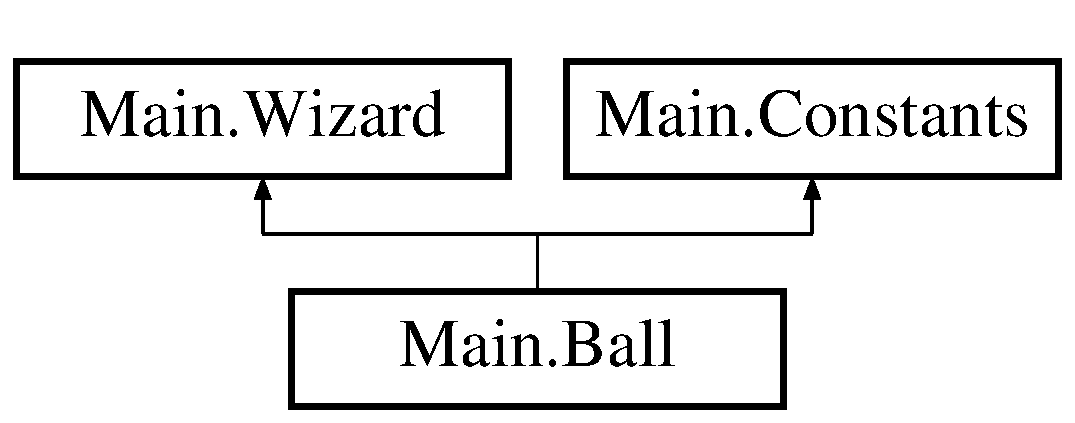
\includegraphics[height=2.000000cm]{class_main_1_1_ball}
\end{center}
\end{figure}
\subsection*{Public Member Functions}
\begin{DoxyCompactItemize}
\item 
\hyperlink{class_main_1_1_ball_a580f1396ea60ed222785d87ae163c5a0}{Ball} ()
\item 
void \hyperlink{class_main_1_1_ball_a00adb8edbc60dacdec6cfac1dd686871}{move} ()
\item 
void \hyperlink{class_main_1_1_ball_a0574633ff91fa6182f8319472208610e}{set\+X\+Direction} (int x)
\item 
int \hyperlink{class_main_1_1_ball_acc35e91c14a087781c30d4ef07ed4883}{get\+X\+Direction} ()
\item 
void \hyperlink{class_main_1_1_ball_a707727e3e5c6fcdb2d06ff438beb7029}{set\+Y\+Direction} (int y)
\item 
int \hyperlink{class_main_1_1_ball_affc1081f609c10e7897ee2da26c81dff}{get\+Y\+Direction} ()
\end{DoxyCompactItemize}
\subsection*{Private Member Functions}
\begin{DoxyCompactItemize}
\item 
void \hyperlink{class_main_1_1_ball_aadbc2f06340363bc41ee7f7646f90460}{reset\+State} ()
\end{DoxyCompactItemize}
\subsection*{Private Attributes}
\begin{DoxyCompactItemize}
\item 
int {\bfseries xdirection}\hypertarget{class_main_1_1_ball_a45d26a9c6639a1b43bf69b983bd70456}{}\label{class_main_1_1_ball_a45d26a9c6639a1b43bf69b983bd70456}

\item 
int {\bfseries ydirection}\hypertarget{class_main_1_1_ball_af586900d4b05b81bc64245a77bf49955}{}\label{class_main_1_1_ball_af586900d4b05b81bc64245a77bf49955}

\end{DoxyCompactItemize}
\subsection*{Additional Inherited Members}


\subsection{Detailed Description}
A labda (\hyperlink{class_main_1_1_ball}{Ball}) elem osztálya. Amely beállítja a labda kiindulási irányát, mozgását, valamint a megfelelő képet hozzárendeli az egyedhez. 

\subsection{Constructor \& Destructor Documentation}
\index{Main\+::\+Ball@{Main\+::\+Ball}!Ball@{Ball}}
\index{Ball@{Ball}!Main\+::\+Ball@{Main\+::\+Ball}}
\subsubsection[{\texorpdfstring{Ball()}{Ball()}}]{\setlength{\rightskip}{0pt plus 5cm}Main.\+Ball.\+Ball (
\begin{DoxyParamCaption}
{}
\end{DoxyParamCaption}
)}\hypertarget{class_main_1_1_ball_a580f1396ea60ed222785d87ae163c5a0}{}\label{class_main_1_1_ball_a580f1396ea60ed222785d87ae163c5a0}
A \hyperlink{class_main_1_1_ball}{Ball} osztály konstruktora, megadja a labda kiindulási irányát, valamint betölti a megfelelő képet. 

\subsection{Member Function Documentation}
\index{Main\+::\+Ball@{Main\+::\+Ball}!get\+X\+Direction@{get\+X\+Direction}}
\index{get\+X\+Direction@{get\+X\+Direction}!Main\+::\+Ball@{Main\+::\+Ball}}
\subsubsection[{\texorpdfstring{get\+X\+Direction()}{getXDirection()}}]{\setlength{\rightskip}{0pt plus 5cm}int Main.\+Ball.\+get\+X\+Direction (
\begin{DoxyParamCaption}
{}
\end{DoxyParamCaption}
)}\hypertarget{class_main_1_1_ball_acc35e91c14a087781c30d4ef07ed4883}{}\label{class_main_1_1_ball_acc35e91c14a087781c30d4ef07ed4883}
Az aktuális x szerinti iránnyal tér vissza. \begin{DoxyReturn}{Returns}
xdirection -\/ x tengely szerinti irány 
\end{DoxyReturn}
\index{Main\+::\+Ball@{Main\+::\+Ball}!get\+Y\+Direction@{get\+Y\+Direction}}
\index{get\+Y\+Direction@{get\+Y\+Direction}!Main\+::\+Ball@{Main\+::\+Ball}}
\subsubsection[{\texorpdfstring{get\+Y\+Direction()}{getYDirection()}}]{\setlength{\rightskip}{0pt plus 5cm}int Main.\+Ball.\+get\+Y\+Direction (
\begin{DoxyParamCaption}
{}
\end{DoxyParamCaption}
)}\hypertarget{class_main_1_1_ball_affc1081f609c10e7897ee2da26c81dff}{}\label{class_main_1_1_ball_affc1081f609c10e7897ee2da26c81dff}
Az aktuális y szerinti iránnyal tér vissza. \begin{DoxyReturn}{Returns}
ydirection -\/ y tengely szerinti irány 
\end{DoxyReturn}
\index{Main\+::\+Ball@{Main\+::\+Ball}!move@{move}}
\index{move@{move}!Main\+::\+Ball@{Main\+::\+Ball}}
\subsubsection[{\texorpdfstring{move()}{move()}}]{\setlength{\rightskip}{0pt plus 5cm}void Main.\+Ball.\+move (
\begin{DoxyParamCaption}
{}
\end{DoxyParamCaption}
)}\hypertarget{class_main_1_1_ball_a00adb8edbc60dacdec6cfac1dd686871}{}\label{class_main_1_1_ball_a00adb8edbc60dacdec6cfac1dd686871}
A labda mozgását szabályozó metódus. Ha a labda falnak ütközik, akkor visszapattan. \index{Main\+::\+Ball@{Main\+::\+Ball}!reset\+State@{reset\+State}}
\index{reset\+State@{reset\+State}!Main\+::\+Ball@{Main\+::\+Ball}}
\subsubsection[{\texorpdfstring{reset\+State()}{resetState()}}]{\setlength{\rightskip}{0pt plus 5cm}void Main.\+Ball.\+reset\+State (
\begin{DoxyParamCaption}
{}
\end{DoxyParamCaption}
)\hspace{0.3cm}{\ttfamily [private]}}\hypertarget{class_main_1_1_ball_aadbc2f06340363bc41ee7f7646f90460}{}\label{class_main_1_1_ball_aadbc2f06340363bc41ee7f7646f90460}
Visszaállítja a labdát a kezdő pozicióba. \index{Main\+::\+Ball@{Main\+::\+Ball}!set\+X\+Direction@{set\+X\+Direction}}
\index{set\+X\+Direction@{set\+X\+Direction}!Main\+::\+Ball@{Main\+::\+Ball}}
\subsubsection[{\texorpdfstring{set\+X\+Direction(int x)}{setXDirection(int x)}}]{\setlength{\rightskip}{0pt plus 5cm}void Main.\+Ball.\+set\+X\+Direction (
\begin{DoxyParamCaption}
\item[{int}]{x}
\end{DoxyParamCaption}
)}\hypertarget{class_main_1_1_ball_a0574633ff91fa6182f8319472208610e}{}\label{class_main_1_1_ball_a0574633ff91fa6182f8319472208610e}
Beállítja a labda x tengely menti irányát az átvett paraméter szerint. 
\begin{DoxyParams}{Parameters}
{\em x} & -\/ A paraméter ami meghatározza az xdirection értékét. \\
\hline
\end{DoxyParams}
\index{Main\+::\+Ball@{Main\+::\+Ball}!set\+Y\+Direction@{set\+Y\+Direction}}
\index{set\+Y\+Direction@{set\+Y\+Direction}!Main\+::\+Ball@{Main\+::\+Ball}}
\subsubsection[{\texorpdfstring{set\+Y\+Direction(int y)}{setYDirection(int y)}}]{\setlength{\rightskip}{0pt plus 5cm}void Main.\+Ball.\+set\+Y\+Direction (
\begin{DoxyParamCaption}
\item[{int}]{y}
\end{DoxyParamCaption}
)}\hypertarget{class_main_1_1_ball_a707727e3e5c6fcdb2d06ff438beb7029}{}\label{class_main_1_1_ball_a707727e3e5c6fcdb2d06ff438beb7029}
Beállítja a labda y tengely menti irányát az átvett paraméter szerint. 
\begin{DoxyParams}{Parameters}
{\em y} & A paraméter ami meghatározza az ydirection értékét. \\
\hline
\end{DoxyParams}


The documentation for this class was generated from the following file\+:\begin{DoxyCompactItemize}
\item 
E\+:/\+Egyetem/\+I\+I. ev/\+I. felev/\+Java/\+H\+F Break Bricks/src/\+Main/Ball.\+java\end{DoxyCompactItemize}

\hypertarget{class_main_1_1_brick}{}\section{Main.\+Brick Class Reference}
\label{class_main_1_1_brick}\index{Main.\+Brick@{Main.\+Brick}}
Inheritance diagram for Main.\+Brick\+:\begin{figure}[H]
\begin{center}
\leavevmode
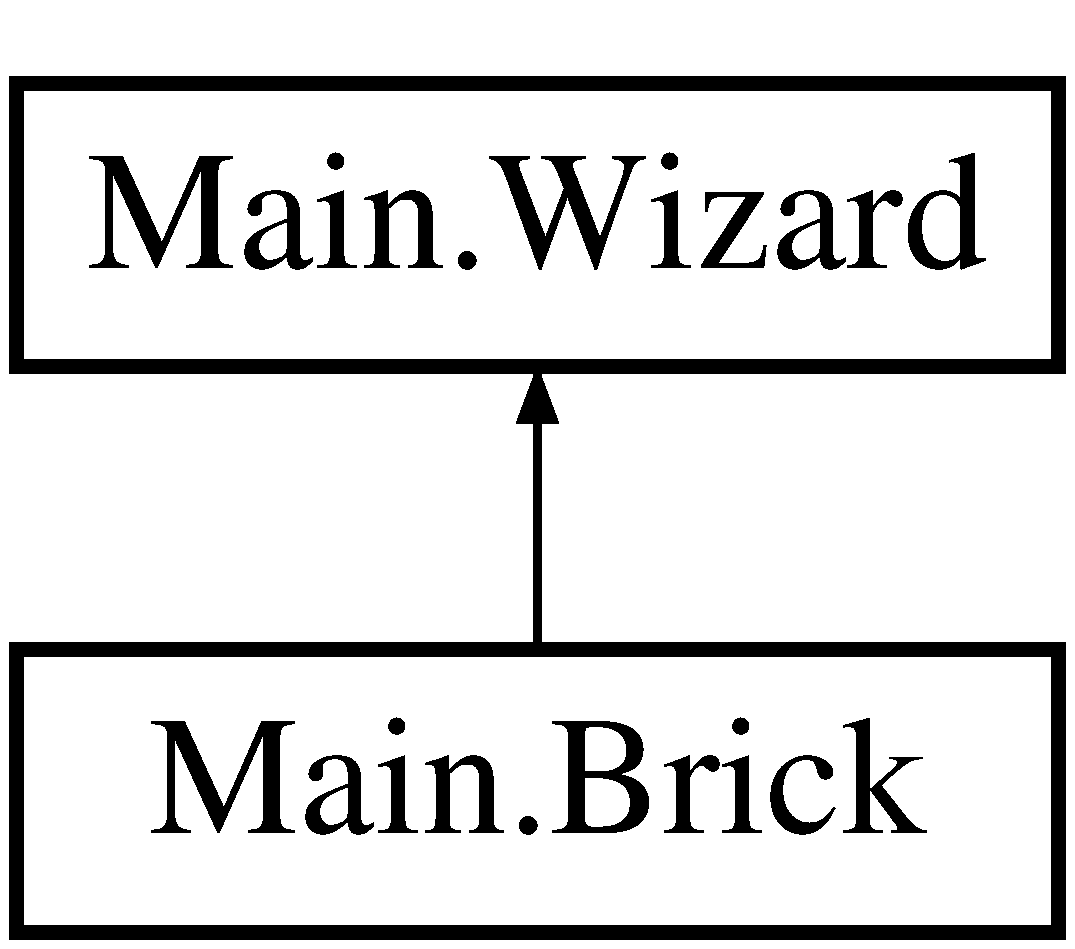
\includegraphics[height=2.000000cm]{class_main_1_1_brick}
\end{center}
\end{figure}
\subsection*{Public Member Functions}
\begin{DoxyCompactItemize}
\item 
\hyperlink{class_main_1_1_brick_a82323322bc85cd2c25936ff7b7fa24c4}{Brick} (int x, int y)
\item 
boolean \hyperlink{class_main_1_1_brick_a0db489a431d39848dbe5bf1a29806d5b}{is\+Destroyed} ()
\item 
void \hyperlink{class_main_1_1_brick_a3308c5fb485ad1c1f2d85bf1fc00d828}{set\+Destroyed} (boolean val)
\end{DoxyCompactItemize}
\subsection*{Private Attributes}
\begin{DoxyCompactItemize}
\item 
boolean {\bfseries destroyed}\hypertarget{class_main_1_1_brick_a0d8384d31b5a1db89e115dfc2517b143}{}\label{class_main_1_1_brick_a0d8384d31b5a1db89e115dfc2517b143}

\end{DoxyCompactItemize}
\subsection*{Additional Inherited Members}


\subsection{Detailed Description}
A tégla (\hyperlink{class_main_1_1_brick}{Brick}) osztály, amely beállítja az adott elemhez rendelt képet, valamint a megjelenítési pozícióját. 

\subsection{Constructor \& Destructor Documentation}
\index{Main\+::\+Brick@{Main\+::\+Brick}!Brick@{Brick}}
\index{Brick@{Brick}!Main\+::\+Brick@{Main\+::\+Brick}}
\subsubsection[{\texorpdfstring{Brick(int x, int y)}{Brick(int x, int y)}}]{\setlength{\rightskip}{0pt plus 5cm}Main.\+Brick.\+Brick (
\begin{DoxyParamCaption}
\item[{int}]{x, }
\item[{int}]{y}
\end{DoxyParamCaption}
)}\hypertarget{class_main_1_1_brick_a82323322bc85cd2c25936ff7b7fa24c4}{}\label{class_main_1_1_brick_a82323322bc85cd2c25936ff7b7fa24c4}
A \hyperlink{class_main_1_1_brick}{Brick} osztály konstruktora, meghatárpzza az adott tégla koordinátáit. 
\begin{DoxyParams}{Parameters}
{\em x} & koordináta értéke \\
\hline
{\em y} & koordináta értéke \\
\hline
\end{DoxyParams}


\subsection{Member Function Documentation}
\index{Main\+::\+Brick@{Main\+::\+Brick}!is\+Destroyed@{is\+Destroyed}}
\index{is\+Destroyed@{is\+Destroyed}!Main\+::\+Brick@{Main\+::\+Brick}}
\subsubsection[{\texorpdfstring{is\+Destroyed()}{isDestroyed()}}]{\setlength{\rightskip}{0pt plus 5cm}boolean Main.\+Brick.\+is\+Destroyed (
\begin{DoxyParamCaption}
{}
\end{DoxyParamCaption}
)}\hypertarget{class_main_1_1_brick_a0db489a431d39848dbe5bf1a29806d5b}{}\label{class_main_1_1_brick_a0db489a431d39848dbe5bf1a29806d5b}
\begin{DoxyReturn}{Returns}
destroyed Visszatér a destroyed logikai változó igazságértékével (true/false). 
\end{DoxyReturn}
\index{Main\+::\+Brick@{Main\+::\+Brick}!set\+Destroyed@{set\+Destroyed}}
\index{set\+Destroyed@{set\+Destroyed}!Main\+::\+Brick@{Main\+::\+Brick}}
\subsubsection[{\texorpdfstring{set\+Destroyed(boolean val)}{setDestroyed(boolean val)}}]{\setlength{\rightskip}{0pt plus 5cm}void Main.\+Brick.\+set\+Destroyed (
\begin{DoxyParamCaption}
\item[{boolean}]{val}
\end{DoxyParamCaption}
)}\hypertarget{class_main_1_1_brick_a3308c5fb485ad1c1f2d85bf1fc00d828}{}\label{class_main_1_1_brick_a3308c5fb485ad1c1f2d85bf1fc00d828}
Beállitha a destroyed logikai változót a megadott igazságérték szerint. 
\begin{DoxyParams}{Parameters}
{\em val} & logikai változó \\
\hline
\end{DoxyParams}


The documentation for this class was generated from the following file\+:\begin{DoxyCompactItemize}
\item 
E\+:/\+Egyetem/\+I\+I. ev/\+I. felev/\+Java/\+H\+F Break Bricks/src/\+Main/Brick.\+java\end{DoxyCompactItemize}

\hypertarget{interface_main_1_1_constants}{}\section{Main.\+Constants Interface Reference}
\label{interface_main_1_1_constants}\index{Main.\+Constants@{Main.\+Constants}}
Inheritance diagram for Main.\+Constants\+:\begin{figure}[H]
\begin{center}
\leavevmode
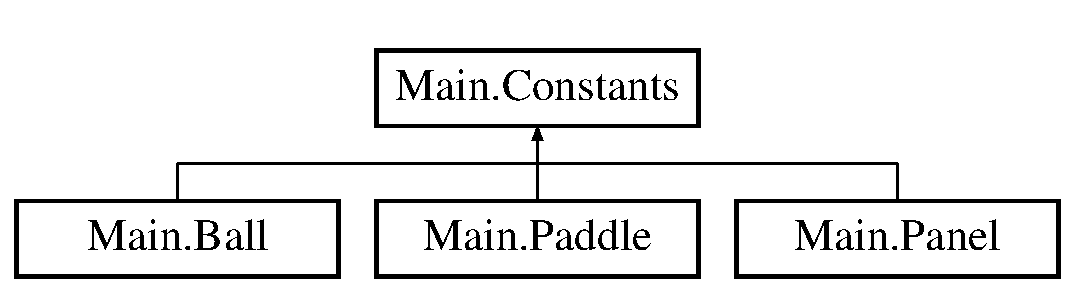
\includegraphics[height=2.000000cm]{interface_main_1_1_constants}
\end{center}
\end{figure}
\subsection*{Static Public Attributes}
\begin{DoxyCompactItemize}
\item 
static final int {\bfseries W\+I\+D\+TH} = 300\hypertarget{interface_main_1_1_constants_aceeaa8dcf3007d8fb01887b7e1d9d5f1}{}\label{interface_main_1_1_constants_aceeaa8dcf3007d8fb01887b7e1d9d5f1}

\item 
static final int {\bfseries H\+E\+I\+G\+HT} = 400\hypertarget{interface_main_1_1_constants_a20e624d65ef606988bf216536879e92e}{}\label{interface_main_1_1_constants_a20e624d65ef606988bf216536879e92e}

\item 
static final int {\bfseries S\+C\+A\+LE} = 2\hypertarget{interface_main_1_1_constants_a5b60bd784179d0dcf0e411c7d1989f2b}{}\label{interface_main_1_1_constants_a5b60bd784179d0dcf0e411c7d1989f2b}

\item 
static final int {\bfseries B\+O\+T\+T\+O\+M\+\_\+\+E\+D\+GE} = 390\hypertarget{interface_main_1_1_constants_a1b98791e45fc64b1d39f1ff475c1ad6b}{}\label{interface_main_1_1_constants_a1b98791e45fc64b1d39f1ff475c1ad6b}

\item 
static final int {\bfseries N\+U\+M\+B\+E\+R\+\_\+\+O\+F\+\_\+\+B\+R\+I\+C\+KS} = 30\hypertarget{interface_main_1_1_constants_acf733ef17154953ae3b34ed500ef95f4}{}\label{interface_main_1_1_constants_acf733ef17154953ae3b34ed500ef95f4}

\item 
static final int {\bfseries S\+T\+A\+R\+T\+\_\+\+P\+O\+S\+\_\+\+P\+A\+D\+D\+L\+E\+\_\+X} = 123\hypertarget{interface_main_1_1_constants_a793d44c56e3dbefda3d0f7b625f9327a}{}\label{interface_main_1_1_constants_a793d44c56e3dbefda3d0f7b625f9327a}

\item 
static final int {\bfseries S\+T\+A\+R\+T\+\_\+\+P\+O\+S\+\_\+\+P\+A\+D\+D\+L\+E\+\_\+Y} = 340\hypertarget{interface_main_1_1_constants_adb7f0a7fae200b50cf3e985a34ce34a6}{}\label{interface_main_1_1_constants_adb7f0a7fae200b50cf3e985a34ce34a6}

\item 
static final int {\bfseries S\+T\+A\+R\+T\+\_\+\+P\+O\+S\+\_\+\+B\+A\+L\+L\+\_\+X} = 140\hypertarget{interface_main_1_1_constants_a8c2ae8584f22b06303575577ef109624}{}\label{interface_main_1_1_constants_a8c2ae8584f22b06303575577ef109624}

\item 
static final int {\bfseries S\+T\+A\+R\+T\+\_\+\+P\+O\+S\+\_\+\+B\+A\+L\+L\+\_\+Y} = 324\hypertarget{interface_main_1_1_constants_ad0e276f2bb956f718629e1f6fa1988e7}{}\label{interface_main_1_1_constants_ad0e276f2bb956f718629e1f6fa1988e7}

\item 
static final int {\bfseries D\+E\+L\+AY} = 1000\hypertarget{interface_main_1_1_constants_a01bea59ae678a38ee578ebc11212f236}{}\label{interface_main_1_1_constants_a01bea59ae678a38ee578ebc11212f236}

\item 
static final int {\bfseries P\+E\+R\+I\+OD} = 7\hypertarget{interface_main_1_1_constants_abb67371ab97c59dda27d443b0b00ba8f}{}\label{interface_main_1_1_constants_abb67371ab97c59dda27d443b0b00ba8f}

\item 
static String {\bfseries T\+I\+T\+LE} = \char`\"{}Break Bricks\char`\"{}\hypertarget{interface_main_1_1_constants_a91b7cff93f92379d2649db9297cf5503}{}\label{interface_main_1_1_constants_a91b7cff93f92379d2649db9297cf5503}

\end{DoxyCompactItemize}


\subsection{Detailed Description}
Created by Előd on 2016.\+11.\+25.. 

The documentation for this interface was generated from the following file\+:\begin{DoxyCompactItemize}
\item 
E\+:/\+Egyetem/\+I\+I. ev/\+I. felev/\+Java/\+H\+F Break Bricks/src/\+Main/Constants.\+java\end{DoxyCompactItemize}

\hypertarget{class_main_1_1_game}{}\section{Main.\+Game Class Reference}
\label{class_main_1_1_game}\index{Main.\+Game@{Main.\+Game}}
\subsection*{Public Member Functions}
\begin{DoxyCompactItemize}
\item 
\hyperlink{class_main_1_1_game_a70ad2e64be2b8ce4b4565fc27eeefeca}{Game} ()
\end{DoxyCompactItemize}
\subsection*{Static Public Member Functions}
\begin{DoxyCompactItemize}
\item 
static void \hyperlink{class_main_1_1_game_ad2487fe3a5117abb92c19fc28f7c952b}{init\+UI} ()
\item 
static void \hyperlink{class_main_1_1_game_aeb69f4b4fba3b270ea8ff820685017e7}{main} (String\mbox{[}$\,$\mbox{]} args)
\end{DoxyCompactItemize}


\subsection{Detailed Description}
A main függvényt tartalmazó osztály, ez indítja el az alkalmazás működését. 

\subsection{Constructor \& Destructor Documentation}
\index{Main\+::\+Game@{Main\+::\+Game}!Game@{Game}}
\index{Game@{Game}!Main\+::\+Game@{Main\+::\+Game}}
\subsubsection[{\texorpdfstring{Game()}{Game()}}]{\setlength{\rightskip}{0pt plus 5cm}Main.\+Game.\+Game (
\begin{DoxyParamCaption}
{}
\end{DoxyParamCaption}
)}\hypertarget{class_main_1_1_game_a70ad2e64be2b8ce4b4565fc27eeefeca}{}\label{class_main_1_1_game_a70ad2e64be2b8ce4b4565fc27eeefeca}
meghívja az \hyperlink{class_main_1_1_game_ad2487fe3a5117abb92c19fc28f7c952b}{init\+U\+I()} függvényt. 

\subsection{Member Function Documentation}
\index{Main\+::\+Game@{Main\+::\+Game}!init\+UI@{init\+UI}}
\index{init\+UI@{init\+UI}!Main\+::\+Game@{Main\+::\+Game}}
\subsubsection[{\texorpdfstring{init\+U\+I()}{initUI()}}]{\setlength{\rightskip}{0pt plus 5cm}static void Main.\+Game.\+init\+UI (
\begin{DoxyParamCaption}
{}
\end{DoxyParamCaption}
)\hspace{0.3cm}{\ttfamily [static]}}\hypertarget{class_main_1_1_game_ad2487fe3a5117abb92c19fc28f7c952b}{}\label{class_main_1_1_game_ad2487fe3a5117abb92c19fc28f7c952b}
Ez a metódus meghatározza azt az ablakot, amelyikben a játék futni fog, és meghívja a \hyperlink{class_main_1_1_panel}{Panel} osztály konstruktorát. Tehát lényegében ennek a függvénynek a hívásával tudjuk elindítani a játékot. \index{Main\+::\+Game@{Main\+::\+Game}!main@{main}}
\index{main@{main}!Main\+::\+Game@{Main\+::\+Game}}
\subsubsection[{\texorpdfstring{main(\+String[] args)}{main(String[] args)}}]{\setlength{\rightskip}{0pt plus 5cm}static void Main.\+Game.\+main (
\begin{DoxyParamCaption}
\item[{String\mbox{[}$\,$\mbox{]}}]{args}
\end{DoxyParamCaption}
)\hspace{0.3cm}{\ttfamily [static]}}\hypertarget{class_main_1_1_game_aeb69f4b4fba3b270ea8ff820685017e7}{}\label{class_main_1_1_game_aeb69f4b4fba3b270ea8ff820685017e7}
A main függvény. Elindítja az alkalmazás működését, egy \hyperlink{class_main_1_1_menu}{Menu} típusú változó létrehozásának a segítségével. 
\begin{DoxyParams}{Parameters}
{\em args} & -\/ main függvény default paramétere \\
\hline
\end{DoxyParams}


The documentation for this class was generated from the following file\+:\begin{DoxyCompactItemize}
\item 
E\+:/\+Egyetem/\+I\+I. ev/\+I. felev/\+Java/\+H\+F Break Bricks/src/\+Main/Game.\+java\end{DoxyCompactItemize}

\hypertarget{class_main_1_1_menu}{}\section{Main.\+Menu Class Reference}
\label{class_main_1_1_menu}\index{Main.\+Menu@{Main.\+Menu}}
Inheritance diagram for Main.\+Menu\+:\begin{figure}[H]
\begin{center}
\leavevmode
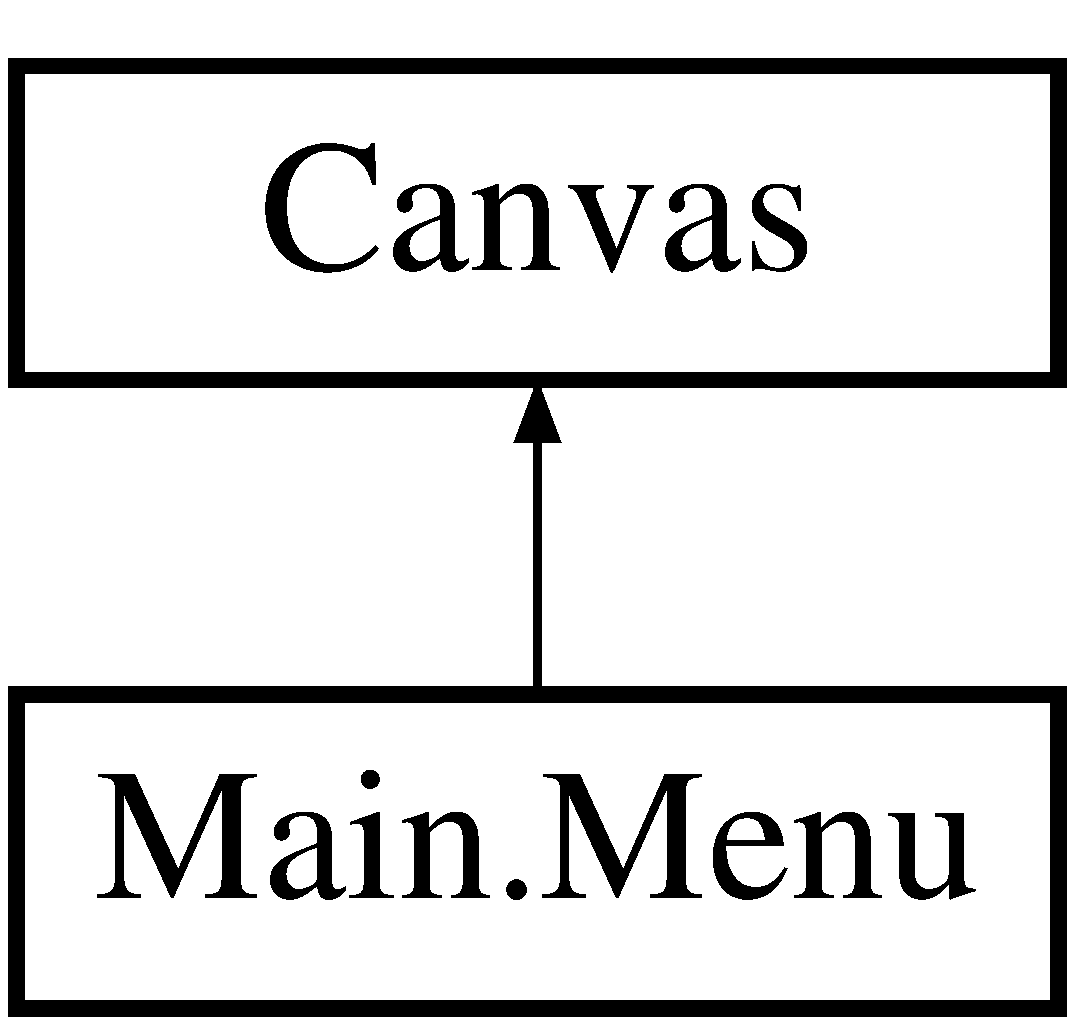
\includegraphics[height=2.000000cm]{class_main_1_1_menu}
\end{center}
\end{figure}
\subsection*{Classes}
\begin{DoxyCompactItemize}
\item 
class \hyperlink{class_main_1_1_menu_1_1_record_listener}{Record\+Listener}
\end{DoxyCompactItemize}
\subsection*{Public Member Functions}
\begin{DoxyCompactItemize}
\item 
\hyperlink{class_main_1_1_menu_a4e9d5494e91330f9588d7f4660733d72}{Menu} ()
\end{DoxyCompactItemize}
\subsection*{Static Public Attributes}
\begin{DoxyCompactItemize}
\item 
static final int {\bfseries W\+I\+D\+TH} = 320\hypertarget{class_main_1_1_menu_aa657c34b78573b6f60e1b5226833d7f8}{}\label{class_main_1_1_menu_aa657c34b78573b6f60e1b5226833d7f8}

\item 
static final int {\bfseries H\+E\+I\+G\+HT} = W\+I\+D\+TH / 12 $\ast$9\hypertarget{class_main_1_1_menu_acfc13d118164d6f5f55f0cc5ab64b2ab}{}\label{class_main_1_1_menu_acfc13d118164d6f5f55f0cc5ab64b2ab}

\item 
static final int {\bfseries S\+C\+A\+LE} = 2\hypertarget{class_main_1_1_menu_aaf4198ccad093c436a2b2f2851475e69}{}\label{class_main_1_1_menu_aaf4198ccad093c436a2b2f2851475e69}

\end{DoxyCompactItemize}
\subsection*{Protected Attributes}
\begin{DoxyCompactItemize}
\item 
Image {\bfseries image}\hypertarget{class_main_1_1_menu_abcb08ae807d5401c995eebad7a6d0cf7}{}\label{class_main_1_1_menu_abcb08ae807d5401c995eebad7a6d0cf7}

\end{DoxyCompactItemize}


\subsection{Detailed Description}
Ez a \hyperlink{class_main_1_1_menu}{Menu} osztályunk, amely a User Interface megvalósítását támogatja. 

\subsection{Constructor \& Destructor Documentation}
\index{Main\+::\+Menu@{Main\+::\+Menu}!Menu@{Menu}}
\index{Menu@{Menu}!Main\+::\+Menu@{Main\+::\+Menu}}
\subsubsection[{\texorpdfstring{Menu()}{Menu()}}]{\setlength{\rightskip}{0pt plus 5cm}Main.\+Menu.\+Menu (
\begin{DoxyParamCaption}
{}
\end{DoxyParamCaption}
)}\hypertarget{class_main_1_1_menu_a4e9d5494e91330f9588d7f4660733d72}{}\label{class_main_1_1_menu_a4e9d5494e91330f9588d7f4660733d72}
A \hyperlink{class_main_1_1_menu}{Menu} osztályunk konstruktora, amely kirajzolja a menünket a képernyőre. Támogatja a menüpontok közötti váltázokat, valamint egy gomb megnyomása segítségével innen indítható a játékonk. Alapvetően 4 opciót tartalmaz\+: Play, Help, \hyperlink{class_main_1_1_records}{Records}, Quit. A Quit gomb megnyomásával ugyan azt a funkciót érhetjük el mint a jobb felső sarokban található x kattintásával, vagyis bezáródik az alkalmazásunk. A \hyperlink{class_main_1_1_records}{Records} menüpont alatt megtekinthető az aktuális top 10-\/es ranglista, amennyiben már van 10 személy a ranglistán. Ha nincs 10 személy, akkor mindenkit megjelenít, aki addig felkerült a listára. A Help menüpont alatt egy rövid útmutató/leírás található a játékhoz. A Play gomb megnyomásával pedig értelemszerűen maga a játék indítható el. A Play gombra való kattintás haátásra elindul a játék egy új ablakban. 
\begin{DoxyParams}{Parameters}
{\em e} & \\
\hline
\end{DoxyParams}
A Help gombra való kattintás hatására megjelenik a játék rövid leírása. 
\begin{DoxyParams}{Parameters}
{\em e} & \\
\hline
\end{DoxyParams}
A Quit gombra kattintva bezárja az alkalmazásunkat. 
\begin{DoxyParams}{Parameters}
{\em e} & \\
\hline
\end{DoxyParams}


The documentation for this class was generated from the following file\+:\begin{DoxyCompactItemize}
\item 
E\+:/\+Egyetem/\+I\+I. ev/\+I. felev/\+Java/\+H\+F Break Bricks/src/\+Main/Menu.\+java\end{DoxyCompactItemize}

\hypertarget{class_main_1_1_paddle}{}\section{Main.\+Paddle Class Reference}
\label{class_main_1_1_paddle}\index{Main.\+Paddle@{Main.\+Paddle}}
Inheritance diagram for Main.\+Paddle\+:\begin{figure}[H]
\begin{center}
\leavevmode
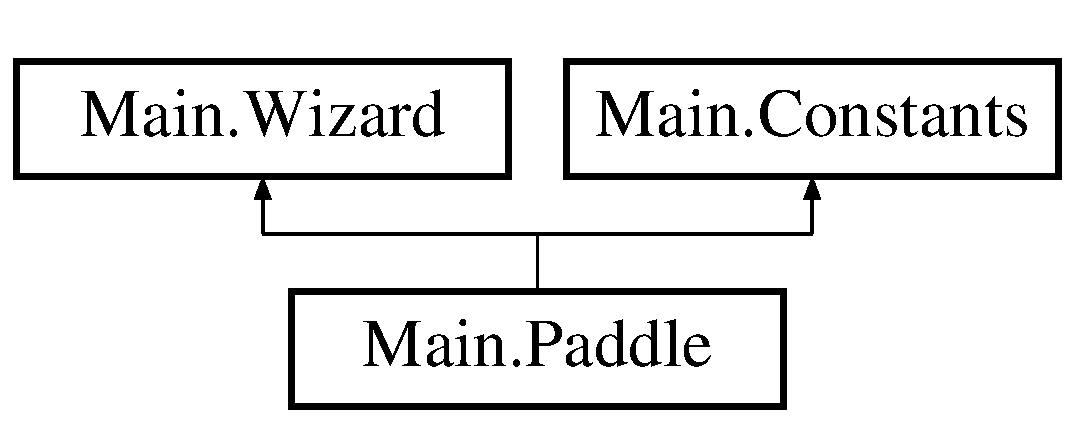
\includegraphics[height=2.000000cm]{class_main_1_1_paddle}
\end{center}
\end{figure}
\subsection*{Public Member Functions}
\begin{DoxyCompactItemize}
\item 
\hyperlink{class_main_1_1_paddle_a06370cc44c3277525cc7f276bfc1d601}{Paddle} ()
\item 
void \hyperlink{class_main_1_1_paddle_ade5930feef33924d190242dfd90e5bc9}{move} ()
\item 
void \hyperlink{class_main_1_1_paddle_adfc1e29e1cdd3df6b4caf75f99471773}{key\+Pressed} (Key\+Event event)
\item 
void \hyperlink{class_main_1_1_paddle_ace7a033051fd52aa4e59f53d9a109be4}{key\+Released} (Key\+Event event)
\end{DoxyCompactItemize}
\subsection*{Private Member Functions}
\begin{DoxyCompactItemize}
\item 
void \hyperlink{class_main_1_1_paddle_a5d6b38c5dc37a6b3f22c64521daf8e99}{reset\+State} ()
\end{DoxyCompactItemize}
\subsection*{Private Attributes}
\begin{DoxyCompactItemize}
\item 
int {\bfseries dx}\hypertarget{class_main_1_1_paddle_af47d4ee4b9d59a39273cc3ec9c8c5a16}{}\label{class_main_1_1_paddle_af47d4ee4b9d59a39273cc3ec9c8c5a16}

\end{DoxyCompactItemize}
\subsection*{Additional Inherited Members}


\subsection{Detailed Description}
A játékos által irányított \hyperlink{class_main_1_1_paddle}{Paddle} (ütő) osztály, az irányításához és beállításához szükséges metódusokkal. 

\subsection{Constructor \& Destructor Documentation}
\index{Main\+::\+Paddle@{Main\+::\+Paddle}!Paddle@{Paddle}}
\index{Paddle@{Paddle}!Main\+::\+Paddle@{Main\+::\+Paddle}}
\subsubsection[{\texorpdfstring{Paddle()}{Paddle()}}]{\setlength{\rightskip}{0pt plus 5cm}Main.\+Paddle.\+Paddle (
\begin{DoxyParamCaption}
{}
\end{DoxyParamCaption}
)}\hypertarget{class_main_1_1_paddle_a06370cc44c3277525cc7f276bfc1d601}{}\label{class_main_1_1_paddle_a06370cc44c3277525cc7f276bfc1d601}
A \hyperlink{class_main_1_1_paddle}{Paddle} (utő) osztály konstruktora. az egyedhez rendeli a képet, valamint beállítja a kiindulási pozicióját. 

\subsection{Member Function Documentation}
\index{Main\+::\+Paddle@{Main\+::\+Paddle}!key\+Pressed@{key\+Pressed}}
\index{key\+Pressed@{key\+Pressed}!Main\+::\+Paddle@{Main\+::\+Paddle}}
\subsubsection[{\texorpdfstring{key\+Pressed(\+Key\+Event event)}{keyPressed(KeyEvent event)}}]{\setlength{\rightskip}{0pt plus 5cm}void Main.\+Paddle.\+key\+Pressed (
\begin{DoxyParamCaption}
\item[{Key\+Event}]{event}
\end{DoxyParamCaption}
)}\hypertarget{class_main_1_1_paddle_adfc1e29e1cdd3df6b4caf75f99471773}{}\label{class_main_1_1_paddle_adfc1e29e1cdd3df6b4caf75f99471773}
Figyeli, hogy melyik gomb lett lenyomva. Balra nyíl esetén balra irányítja az ütőt. Jobbra nyíl lenyomása esetén pedig jobbra. 
\begin{DoxyParams}{Parameters}
{\em event} & Key\+Event beépített osztály paramétere \\
\hline
\end{DoxyParams}
\index{Main\+::\+Paddle@{Main\+::\+Paddle}!key\+Released@{key\+Released}}
\index{key\+Released@{key\+Released}!Main\+::\+Paddle@{Main\+::\+Paddle}}
\subsubsection[{\texorpdfstring{key\+Released(\+Key\+Event event)}{keyReleased(KeyEvent event)}}]{\setlength{\rightskip}{0pt plus 5cm}void Main.\+Paddle.\+key\+Released (
\begin{DoxyParamCaption}
\item[{Key\+Event}]{event}
\end{DoxyParamCaption}
)}\hypertarget{class_main_1_1_paddle_ace7a033051fd52aa4e59f53d9a109be4}{}\label{class_main_1_1_paddle_ace7a033051fd52aa4e59f53d9a109be4}
Figyeli a lenyomott billenytyű felengedését. Ha felengedtük a lenyomott gombot, akkor megáll az ütő egyhelyben. 
\begin{DoxyParams}{Parameters}
{\em event} & Key\+Event beépített osztály paramétere \\
\hline
\end{DoxyParams}
\index{Main\+::\+Paddle@{Main\+::\+Paddle}!move@{move}}
\index{move@{move}!Main\+::\+Paddle@{Main\+::\+Paddle}}
\subsubsection[{\texorpdfstring{move()}{move()}}]{\setlength{\rightskip}{0pt plus 5cm}void Main.\+Paddle.\+move (
\begin{DoxyParamCaption}
{}
\end{DoxyParamCaption}
)}\hypertarget{class_main_1_1_paddle_ade5930feef33924d190242dfd90e5bc9}{}\label{class_main_1_1_paddle_ade5930feef33924d190242dfd90e5bc9}
Az utő mozgását szabályozza. Kizárólag x tengely szerint tud működni, és nem tud kimenni az ablakból. A szélénél megütközik. \index{Main\+::\+Paddle@{Main\+::\+Paddle}!reset\+State@{reset\+State}}
\index{reset\+State@{reset\+State}!Main\+::\+Paddle@{Main\+::\+Paddle}}
\subsubsection[{\texorpdfstring{reset\+State()}{resetState()}}]{\setlength{\rightskip}{0pt plus 5cm}void Main.\+Paddle.\+reset\+State (
\begin{DoxyParamCaption}
{}
\end{DoxyParamCaption}
)\hspace{0.3cm}{\ttfamily [private]}}\hypertarget{class_main_1_1_paddle_a5d6b38c5dc37a6b3f22c64521daf8e99}{}\label{class_main_1_1_paddle_a5d6b38c5dc37a6b3f22c64521daf8e99}
Visszaállítja az ütő koordinátáit a kezdőpozícióba. 

The documentation for this class was generated from the following file\+:\begin{DoxyCompactItemize}
\item 
E\+:/\+Egyetem/\+I\+I. ev/\+I. felev/\+Java/\+H\+F Break Bricks/src/\+Main/Paddle.\+java\end{DoxyCompactItemize}

\hypertarget{class_main_1_1_panel}{}\section{Main.\+Panel Class Reference}
\label{class_main_1_1_panel}\index{Main.\+Panel@{Main.\+Panel}}
Inheritance diagram for Main.\+Panel\+:\begin{figure}[H]
\begin{center}
\leavevmode
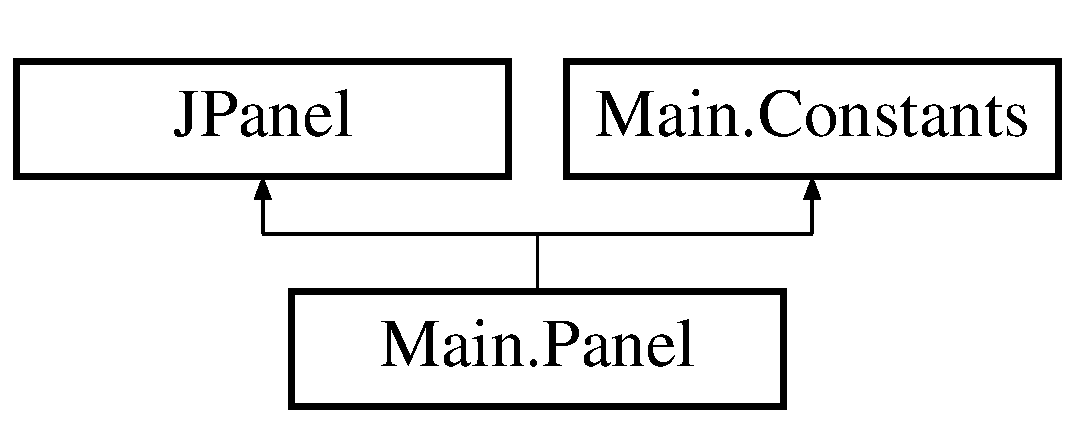
\includegraphics[height=2.000000cm]{class_main_1_1_panel}
\end{center}
\end{figure}
\subsection*{Classes}
\begin{DoxyCompactItemize}
\item 
class \hyperlink{class_main_1_1_panel_1_1_schedule_task}{Schedule\+Task}
\item 
class \hyperlink{class_main_1_1_panel_1_1_t_adapter}{T\+Adapter}
\end{DoxyCompactItemize}
\subsection*{Public Member Functions}
\begin{DoxyCompactItemize}
\item 
\hyperlink{class_main_1_1_panel_a1e24432e564f9ce3ba9256b62b747f49}{Panel} ()
\item 
void \hyperlink{class_main_1_1_panel_a43135c9d6be14c228f7c530613f9fd87}{add\+Notify} ()
\item 
void \hyperlink{class_main_1_1_panel_a99b5a8bb204915a0fe15c62762434838}{create} ()
\item 
void \hyperlink{class_main_1_1_panel_a6903271f2f5062667ff01b3d1d748cb7}{paint\+Component} (Graphics g)
\item 
void \hyperlink{class_main_1_1_panel_a4abb223924af2b3ff64bae87a74644bf}{game\+Over} (Graphics2D g2d)
\end{DoxyCompactItemize}
\subsection*{Public Attributes}
\begin{DoxyCompactItemize}
\item 
Array\+List$<$ \hyperlink{class_main_1_1_records}{Records} $>$ {\bfseries records} = new Array\+List$<$$>$()\hypertarget{class_main_1_1_panel_a1316464998129458ce372c8148dca5c6}{}\label{class_main_1_1_panel_a1316464998129458ce372c8148dca5c6}

\item 
int {\bfseries count} = 0\hypertarget{class_main_1_1_panel_a0e04764160c5a402424d3ab67aa32bc9}{}\label{class_main_1_1_panel_a0e04764160c5a402424d3ab67aa32bc9}

\end{DoxyCompactItemize}
\subsection*{Private Member Functions}
\begin{DoxyCompactItemize}
\item 
void \hyperlink{class_main_1_1_panel_a765d0ade3fdbb19e9521086296e50655}{init\+Game} ()
\item 
void \hyperlink{class_main_1_1_panel_ab9cc3da060f155580e32bbd8cec3b159}{draw\+Things} (Graphics2D g2d)
\item 
void \hyperlink{class_main_1_1_panel_a533066171c505729288775a25d0e2b8b}{stop\+Game} ()
\item 
void \hyperlink{class_main_1_1_panel_aab0094c5b9b7af46239e23dd646e2dc9}{check\+Collision} ()
\end{DoxyCompactItemize}
\subsection*{Private Attributes}
\begin{DoxyCompactItemize}
\item 
\hyperlink{class_main_1_1_ball}{Ball} {\bfseries ball}\hypertarget{class_main_1_1_panel_a99783cc33bc9f6afba73d36605d7b391}{}\label{class_main_1_1_panel_a99783cc33bc9f6afba73d36605d7b391}

\item 
String {\bfseries message} = \char`\"{}Game Over\char`\"{}\hypertarget{class_main_1_1_panel_a426ef03a02527f18a2bb122c623f9dd1}{}\label{class_main_1_1_panel_a426ef03a02527f18a2bb122c623f9dd1}

\item 
Timer {\bfseries timer}\hypertarget{class_main_1_1_panel_a8a2b9dd3079d409d03ca212ef3eb98df}{}\label{class_main_1_1_panel_a8a2b9dd3079d409d03ca212ef3eb98df}

\item 
Timer {\bfseries timer2}\hypertarget{class_main_1_1_panel_a749ae740aab86aaf62e5a76009b60978}{}\label{class_main_1_1_panel_a749ae740aab86aaf62e5a76009b60978}

\item 
\hyperlink{class_main_1_1_brick}{Brick} {\bfseries bricks} \mbox{[}$\,$\mbox{]}\hypertarget{class_main_1_1_panel_acafb3c641a56dc6e3c60bbf61c4b160d}{}\label{class_main_1_1_panel_acafb3c641a56dc6e3c60bbf61c4b160d}

\item 
\hyperlink{class_main_1_1_paddle}{Paddle} {\bfseries paddle}\hypertarget{class_main_1_1_panel_a7732f40ed71e4760c0d3e42cb29ebd31}{}\label{class_main_1_1_panel_a7732f40ed71e4760c0d3e42cb29ebd31}

\item 
boolean {\bfseries ingame} = true\hypertarget{class_main_1_1_panel_a22f6b9585a0179a20a84f5d16a335489}{}\label{class_main_1_1_panel_a22f6b9585a0179a20a84f5d16a335489}

\end{DoxyCompactItemize}
\subsection*{Additional Inherited Members}


\subsection{Detailed Description}
Ez a \hyperlink{class_main_1_1_panel}{Panel} osztály, amely lényegében kiíratja az objektumokat a képernyőre, figyeli azok viselkedését, és ezek alapján folyamatosan újrarajzolja őket. Lényegében ez az osztály vezérli a játék működését. 

\subsection{Constructor \& Destructor Documentation}
\index{Main\+::\+Panel@{Main\+::\+Panel}!Panel@{Panel}}
\index{Panel@{Panel}!Main\+::\+Panel@{Main\+::\+Panel}}
\subsubsection[{\texorpdfstring{Panel()}{Panel()}}]{\setlength{\rightskip}{0pt plus 5cm}Main.\+Panel.\+Panel (
\begin{DoxyParamCaption}
{}
\end{DoxyParamCaption}
)}\hypertarget{class_main_1_1_panel_a1e24432e564f9ce3ba9256b62b747f49}{}\label{class_main_1_1_panel_a1e24432e564f9ce3ba9256b62b747f49}
Az osztály konstruktora, meghívja az inicialisáló metódust. 

\subsection{Member Function Documentation}
\index{Main\+::\+Panel@{Main\+::\+Panel}!add\+Notify@{add\+Notify}}
\index{add\+Notify@{add\+Notify}!Main\+::\+Panel@{Main\+::\+Panel}}
\subsubsection[{\texorpdfstring{add\+Notify()}{addNotify()}}]{\setlength{\rightskip}{0pt plus 5cm}void Main.\+Panel.\+add\+Notify (
\begin{DoxyParamCaption}
{}
\end{DoxyParamCaption}
)}\hypertarget{class_main_1_1_panel_a43135c9d6be14c228f7c530613f9fd87}{}\label{class_main_1_1_panel_a43135c9d6be14c228f7c530613f9fd87}
Meghívja a \hyperlink{class_main_1_1_panel_a99b5a8bb204915a0fe15c62762434838}{create()} függvényt. \index{Main\+::\+Panel@{Main\+::\+Panel}!check\+Collision@{check\+Collision}}
\index{check\+Collision@{check\+Collision}!Main\+::\+Panel@{Main\+::\+Panel}}
\subsubsection[{\texorpdfstring{check\+Collision()}{checkCollision()}}]{\setlength{\rightskip}{0pt plus 5cm}void Main.\+Panel.\+check\+Collision (
\begin{DoxyParamCaption}
{}
\end{DoxyParamCaption}
)\hspace{0.3cm}{\ttfamily [private]}}\hypertarget{class_main_1_1_panel_aab0094c5b9b7af46239e23dd646e2dc9}{}\label{class_main_1_1_panel_aab0094c5b9b7af46239e23dd646e2dc9}
Vizsgálja a játék folyamata közben történt eseményeket. Ha téglámak ötküzik, akkor eltűnteti az adott téglát, a labda pedig visszapattan a megváltott iránya szerint. Ha az ütőnek ütközik, akkor is visszapattan, közben megváltoztatja irányát. Amennyiben a labda eléri az ablak alját, a játék leáll, és a játékosunk veszített. \index{Main\+::\+Panel@{Main\+::\+Panel}!create@{create}}
\index{create@{create}!Main\+::\+Panel@{Main\+::\+Panel}}
\subsubsection[{\texorpdfstring{create()}{create()}}]{\setlength{\rightskip}{0pt plus 5cm}void Main.\+Panel.\+create (
\begin{DoxyParamCaption}
{}
\end{DoxyParamCaption}
)}\hypertarget{class_main_1_1_panel_a99b5a8bb204915a0fe15c62762434838}{}\label{class_main_1_1_panel_a99b5a8bb204915a0fe15c62762434838}
Létrehozza a játékhoz szükséges labdát, ütőt, valamint téglákat, azok helyének meghatározásával. \index{Main\+::\+Panel@{Main\+::\+Panel}!draw\+Things@{draw\+Things}}
\index{draw\+Things@{draw\+Things}!Main\+::\+Panel@{Main\+::\+Panel}}
\subsubsection[{\texorpdfstring{draw\+Things(\+Graphics2\+D g2d)}{drawThings(Graphics2D g2d)}}]{\setlength{\rightskip}{0pt plus 5cm}void Main.\+Panel.\+draw\+Things (
\begin{DoxyParamCaption}
\item[{Graphics2D}]{g2d}
\end{DoxyParamCaption}
)\hspace{0.3cm}{\ttfamily [private]}}\hypertarget{class_main_1_1_panel_ab9cc3da060f155580e32bbd8cec3b159}{}\label{class_main_1_1_panel_ab9cc3da060f155580e32bbd8cec3b159}
Kirajzolja a képernyőre a megfelelő ablakba, a megfelelő helyekre a játék objektumait. 
\begin{DoxyParams}{Parameters}
{\em g2d} & A képernyőre történő kiírást támogatja. \\
\hline
\end{DoxyParams}
\index{Main\+::\+Panel@{Main\+::\+Panel}!game\+Over@{game\+Over}}
\index{game\+Over@{game\+Over}!Main\+::\+Panel@{Main\+::\+Panel}}
\subsubsection[{\texorpdfstring{game\+Over(\+Graphics2\+D g2d)}{gameOver(Graphics2D g2d)}}]{\setlength{\rightskip}{0pt plus 5cm}void Main.\+Panel.\+game\+Over (
\begin{DoxyParamCaption}
\item[{Graphics2D}]{g2d}
\end{DoxyParamCaption}
)}\hypertarget{class_main_1_1_panel_a4abb223924af2b3ff64bae87a74644bf}{}\label{class_main_1_1_panel_a4abb223924af2b3ff64bae87a74644bf}
A játék végkimenetele alapján szabályozza, hogy mi történjen azt követően. Ha a játékos veszít, akkor egy \char`\"{}\+Sajnáljuk ön veszített\char`\"{} felirat fogadja, majd lehetősége van új játék indítására. Amennyiben a játékos sikeresen vette az akadályokat. Akkor egy \char`\"{}\+Victory\char`\"{} felirat után megadhatja a nevét, amelyet a program egy ranglistába tárol a játékidő alapján. 
\begin{DoxyParams}{Parameters}
{\em g2d} & A képernyőre történő kiírást támogatja. \\
\hline
\end{DoxyParams}
\index{Main\+::\+Panel@{Main\+::\+Panel}!init\+Game@{init\+Game}}
\index{init\+Game@{init\+Game}!Main\+::\+Panel@{Main\+::\+Panel}}
\subsubsection[{\texorpdfstring{init\+Game()}{initGame()}}]{\setlength{\rightskip}{0pt plus 5cm}void Main.\+Panel.\+init\+Game (
\begin{DoxyParamCaption}
{}
\end{DoxyParamCaption}
)\hspace{0.3cm}{\ttfamily [private]}}\hypertarget{class_main_1_1_panel_a765d0ade3fdbb19e9521086296e50655}{}\label{class_main_1_1_panel_a765d0ade3fdbb19e9521086296e50655}
Ez a metódus inicializálja a játékhoz szökséges változókat. Megadja a téglák számát, elindít egy belső timert, vagyis esetünkben kettőt. Egyiket a játék periódusidejével, egy másikat pedig 1000ms -\/os periódusidővel, hogy meg tudjuk határozni a játékos játékban töltött idejét. \index{Main\+::\+Panel@{Main\+::\+Panel}!paint\+Component@{paint\+Component}}
\index{paint\+Component@{paint\+Component}!Main\+::\+Panel@{Main\+::\+Panel}}
\subsubsection[{\texorpdfstring{paint\+Component(\+Graphics g)}{paintComponent(Graphics g)}}]{\setlength{\rightskip}{0pt plus 5cm}void Main.\+Panel.\+paint\+Component (
\begin{DoxyParamCaption}
\item[{Graphics}]{g}
\end{DoxyParamCaption}
)}\hypertarget{class_main_1_1_panel_a6903271f2f5062667ff01b3d1d748cb7}{}\label{class_main_1_1_panel_a6903271f2f5062667ff01b3d1d748cb7}
Ha játékban vagyunk, akkor hívja a \hyperlink{class_main_1_1_panel_ab9cc3da060f155580e32bbd8cec3b159}{draw\+Things()} metódust, ha a játéknak vége akkor pedig a \hyperlink{class_main_1_1_panel_a4abb223924af2b3ff64bae87a74644bf}{game\+Over()} metódust. 
\begin{DoxyParams}{Parameters}
{\em g} & A képernyőre történő kiírást támogatja. \\
\hline
\end{DoxyParams}
\index{Main\+::\+Panel@{Main\+::\+Panel}!stop\+Game@{stop\+Game}}
\index{stop\+Game@{stop\+Game}!Main\+::\+Panel@{Main\+::\+Panel}}
\subsubsection[{\texorpdfstring{stop\+Game()}{stopGame()}}]{\setlength{\rightskip}{0pt plus 5cm}void Main.\+Panel.\+stop\+Game (
\begin{DoxyParamCaption}
{}
\end{DoxyParamCaption}
)\hspace{0.3cm}{\ttfamily [private]}}\hypertarget{class_main_1_1_panel_a533066171c505729288775a25d0e2b8b}{}\label{class_main_1_1_panel_a533066171c505729288775a25d0e2b8b}
Leállítja a játékot. 

The documentation for this class was generated from the following file\+:\begin{DoxyCompactItemize}
\item 
E\+:/\+Egyetem/\+I\+I. ev/\+I. felev/\+Java/\+H\+F Break Bricks/src/\+Main/Panel.\+java\end{DoxyCompactItemize}

\hypertarget{class_main_1_1_menu_1_1_record_listener}{}\section{Main.\+Menu.\+Record\+Listener Class Reference}
\label{class_main_1_1_menu_1_1_record_listener}\index{Main.\+Menu.\+Record\+Listener@{Main.\+Menu.\+Record\+Listener}}
Inheritance diagram for Main.\+Menu.\+Record\+Listener\+:\begin{figure}[H]
\begin{center}
\leavevmode
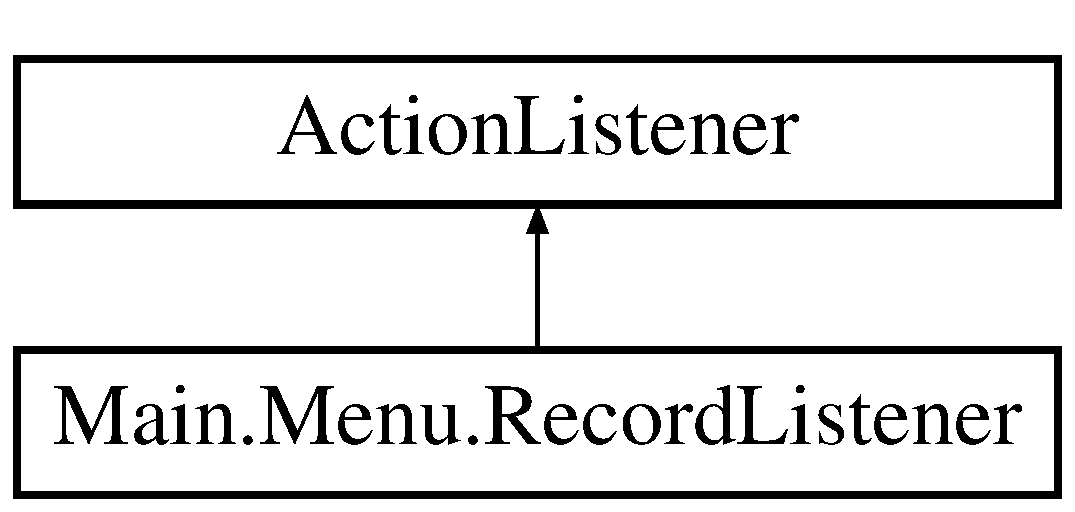
\includegraphics[height=2.000000cm]{class_main_1_1_menu_1_1_record_listener}
\end{center}
\end{figure}
\subsection*{Public Member Functions}
\begin{DoxyCompactItemize}
\item 
void \hyperlink{class_main_1_1_menu_1_1_record_listener_a9268103c16eb0ffe66588255b10b6dee}{action\+Performed} (Action\+Event e)
\end{DoxyCompactItemize}


\subsection{Detailed Description}
Segédosztály, a Record gomb megnyomásával kiváltott történések támogatására. 

\subsection{Member Function Documentation}
\index{Main\+::\+Menu\+::\+Record\+Listener@{Main\+::\+Menu\+::\+Record\+Listener}!action\+Performed@{action\+Performed}}
\index{action\+Performed@{action\+Performed}!Main\+::\+Menu\+::\+Record\+Listener@{Main\+::\+Menu\+::\+Record\+Listener}}
\subsubsection[{\texorpdfstring{action\+Performed(\+Action\+Event e)}{actionPerformed(ActionEvent e)}}]{\setlength{\rightskip}{0pt plus 5cm}void Main.\+Menu.\+Record\+Listener.\+action\+Performed (
\begin{DoxyParamCaption}
\item[{Action\+Event}]{e}
\end{DoxyParamCaption}
)}\hypertarget{class_main_1_1_menu_1_1_record_listener_a9268103c16eb0ffe66588255b10b6dee}{}\label{class_main_1_1_menu_1_1_record_listener_a9268103c16eb0ffe66588255b10b6dee}
Ha a menüben rákattintottunk a \hyperlink{class_main_1_1_records}{Records} gombra, akkor betölti az annak megfelelő ablakot, így láthatjuk és kiovlashatjuk a toplistát. 
\begin{DoxyParams}{Parameters}
{\em e} & \\
\hline
\end{DoxyParams}


The documentation for this class was generated from the following file\+:\begin{DoxyCompactItemize}
\item 
E\+:/\+Egyetem/\+I\+I. ev/\+I. felev/\+Java/\+H\+F Break Bricks/src/\+Main/Menu.\+java\end{DoxyCompactItemize}

\hypertarget{class_main_1_1_records}{}\section{Main.\+Records Class Reference}
\label{class_main_1_1_records}\index{Main.\+Records@{Main.\+Records}}
Inheritance diagram for Main.\+Records\+:\begin{figure}[H]
\begin{center}
\leavevmode
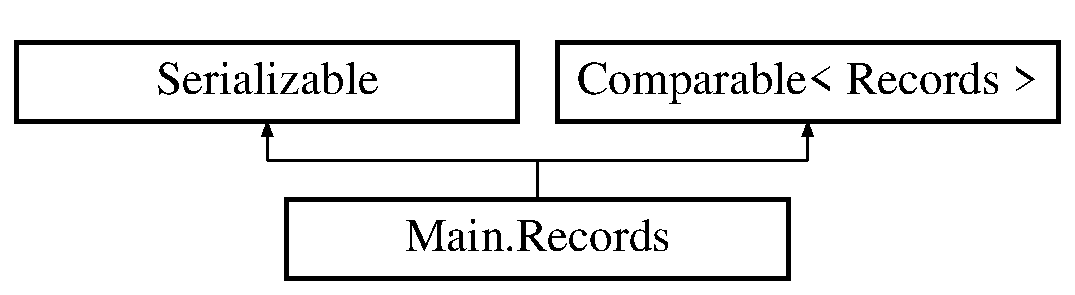
\includegraphics[height=2.000000cm]{class_main_1_1_records}
\end{center}
\end{figure}
\subsection*{Public Member Functions}
\begin{DoxyCompactItemize}
\item 
\hyperlink{class_main_1_1_records_a82bb250f41e6d1cbad9c9d520772d238}{Records} (String name, int score)
\item 
void \hyperlink{class_main_1_1_records_ac1c5fc940f98770509ba2bf237e5ea0b}{write\+Object} (Object\+Output\+Stream oos)
\item 
void \hyperlink{class_main_1_1_records_a78fec3236933217b223e93e5c6eb34d7}{read\+Object} (Object\+Input\+Stream ois)
\item 
String \hyperlink{class_main_1_1_records_ac6f93eb98cdd21d52294c4d90dc76d99}{get\+Name} ()
\item 
int \hyperlink{class_main_1_1_records_a97027b0438ca6123ccda8330987d0174}{get\+Score} ()
\item 
int \hyperlink{class_main_1_1_records_ab5fde5dd0ad92223abbed30c7b22f607}{compare\+To} (\hyperlink{class_main_1_1_records}{Records} r)
\end{DoxyCompactItemize}
\subsection*{Private Attributes}
\begin{DoxyCompactItemize}
\item 
String {\bfseries name}\hypertarget{class_main_1_1_records_a3658db92b27c25c237f903c01afa6443}{}\label{class_main_1_1_records_a3658db92b27c25c237f903c01afa6443}

\item 
int {\bfseries score}\hypertarget{class_main_1_1_records_ad514b8ec841175bb98b168c63753f493}{}\label{class_main_1_1_records_ad514b8ec841175bb98b168c63753f493}

\end{DoxyCompactItemize}


\subsection{Detailed Description}
Lényegében egy segédosztály, amely a ranglistánk fájlba írását, illetve fájlból történő beolvasását támogatja. 

\subsection{Constructor \& Destructor Documentation}
\index{Main\+::\+Records@{Main\+::\+Records}!Records@{Records}}
\index{Records@{Records}!Main\+::\+Records@{Main\+::\+Records}}
\subsubsection[{\texorpdfstring{Records(\+String name, int score)}{Records(String name, int score)}}]{\setlength{\rightskip}{0pt plus 5cm}Main.\+Records.\+Records (
\begin{DoxyParamCaption}
\item[{String}]{name, }
\item[{int}]{score}
\end{DoxyParamCaption}
)}\hypertarget{class_main_1_1_records_a82bb250f41e6d1cbad9c9d520772d238}{}\label{class_main_1_1_records_a82bb250f41e6d1cbad9c9d520772d238}
Az osztályunk konstruktora, meghatározza a paramétereit, a megadott értékek alapján. 
\begin{DoxyParams}{Parameters}
{\em name} & A játékos nevét tárolja. \\
\hline
{\em score} & A játékoshoz és az adott játékhoz tartozó időt méri \\
\hline
\end{DoxyParams}


\subsection{Member Function Documentation}
\index{Main\+::\+Records@{Main\+::\+Records}!compare\+To@{compare\+To}}
\index{compare\+To@{compare\+To}!Main\+::\+Records@{Main\+::\+Records}}
\subsubsection[{\texorpdfstring{compare\+To(\+Records r)}{compareTo(Records r)}}]{\setlength{\rightskip}{0pt plus 5cm}int Main.\+Records.\+compare\+To (
\begin{DoxyParamCaption}
\item[{{\bf Records}}]{r}
\end{DoxyParamCaption}
)}\hypertarget{class_main_1_1_records_ab5fde5dd0ad92223abbed30c7b22f607}{}\label{class_main_1_1_records_ab5fde5dd0ad92223abbed30c7b22f607}
Az adatok count paramétere szerinti sorrendezett tárolást támogató metódus. 
\begin{DoxyParams}{Parameters}
{\em r} & Egy Record típusú változó \\
\hline
\end{DoxyParams}
\begin{DoxyReturn}{Returns}
-\/1, ha az aktuális idő nagyobb mint amihez épp hasonlítjuk 1, ha kisebb 0, különben. 
\end{DoxyReturn}
\index{Main\+::\+Records@{Main\+::\+Records}!get\+Name@{get\+Name}}
\index{get\+Name@{get\+Name}!Main\+::\+Records@{Main\+::\+Records}}
\subsubsection[{\texorpdfstring{get\+Name()}{getName()}}]{\setlength{\rightskip}{0pt plus 5cm}String Main.\+Records.\+get\+Name (
\begin{DoxyParamCaption}
{}
\end{DoxyParamCaption}
)}\hypertarget{class_main_1_1_records_ac6f93eb98cdd21d52294c4d90dc76d99}{}\label{class_main_1_1_records_ac6f93eb98cdd21d52294c4d90dc76d99}
Getter\+: a name paraméter értékével tér vissza. \begin{DoxyReturn}{Returns}
name -\/ Visszatér a játékos nevével. 
\end{DoxyReturn}
\index{Main\+::\+Records@{Main\+::\+Records}!get\+Score@{get\+Score}}
\index{get\+Score@{get\+Score}!Main\+::\+Records@{Main\+::\+Records}}
\subsubsection[{\texorpdfstring{get\+Score()}{getScore()}}]{\setlength{\rightskip}{0pt plus 5cm}int Main.\+Records.\+get\+Score (
\begin{DoxyParamCaption}
{}
\end{DoxyParamCaption}
)}\hypertarget{class_main_1_1_records_a97027b0438ca6123ccda8330987d0174}{}\label{class_main_1_1_records_a97027b0438ca6123ccda8330987d0174}
Getter\+: a score paraméter értékével tér vissza. \begin{DoxyReturn}{Returns}
score -\/ Visszatér a játékos idejével. 
\end{DoxyReturn}
\index{Main\+::\+Records@{Main\+::\+Records}!read\+Object@{read\+Object}}
\index{read\+Object@{read\+Object}!Main\+::\+Records@{Main\+::\+Records}}
\subsubsection[{\texorpdfstring{read\+Object(\+Object\+Input\+Stream ois)}{readObject(ObjectInputStream ois)}}]{\setlength{\rightskip}{0pt plus 5cm}void Main.\+Records.\+read\+Object (
\begin{DoxyParamCaption}
\item[{Object\+Input\+Stream}]{ois}
\end{DoxyParamCaption}
)}\hypertarget{class_main_1_1_records_a78fec3236933217b223e93e5c6eb34d7}{}\label{class_main_1_1_records_a78fec3236933217b223e93e5c6eb34d7}
Egy adott rekord (mint egyed/elem) fájlból történő beolvasását valósítja meg. 
\begin{DoxyParams}{Parameters}
{\em ois} & Object\+Input\+Stream paraméter, a fájlból olvasást támogatja. \\
\hline
\end{DoxyParams}
\index{Main\+::\+Records@{Main\+::\+Records}!write\+Object@{write\+Object}}
\index{write\+Object@{write\+Object}!Main\+::\+Records@{Main\+::\+Records}}
\subsubsection[{\texorpdfstring{write\+Object(\+Object\+Output\+Stream oos)}{writeObject(ObjectOutputStream oos)}}]{\setlength{\rightskip}{0pt plus 5cm}void Main.\+Records.\+write\+Object (
\begin{DoxyParamCaption}
\item[{Object\+Output\+Stream}]{oos}
\end{DoxyParamCaption}
)}\hypertarget{class_main_1_1_records_ac1c5fc940f98770509ba2bf237e5ea0b}{}\label{class_main_1_1_records_ac1c5fc940f98770509ba2bf237e5ea0b}
A kapott elemhez tartozó adatok fájlba írását valósítja meg ez a metódus. 
\begin{DoxyParams}{Parameters}
{\em oos} & Object\+Output\+Stream paraméter, a fájlba írást támogatja. \\
\hline
\end{DoxyParams}


The documentation for this class was generated from the following file\+:\begin{DoxyCompactItemize}
\item 
E\+:/\+Egyetem/\+I\+I. ev/\+I. felev/\+Java/\+H\+F Break Bricks/src/\+Main/Records.\+java\end{DoxyCompactItemize}

\hypertarget{class_main_1_1_panel_1_1_schedule_task}{}\section{Main.\+Panel.\+Schedule\+Task Class Reference}
\label{class_main_1_1_panel_1_1_schedule_task}\index{Main.\+Panel.\+Schedule\+Task@{Main.\+Panel.\+Schedule\+Task}}
Inheritance diagram for Main.\+Panel.\+Schedule\+Task\+:\begin{figure}[H]
\begin{center}
\leavevmode
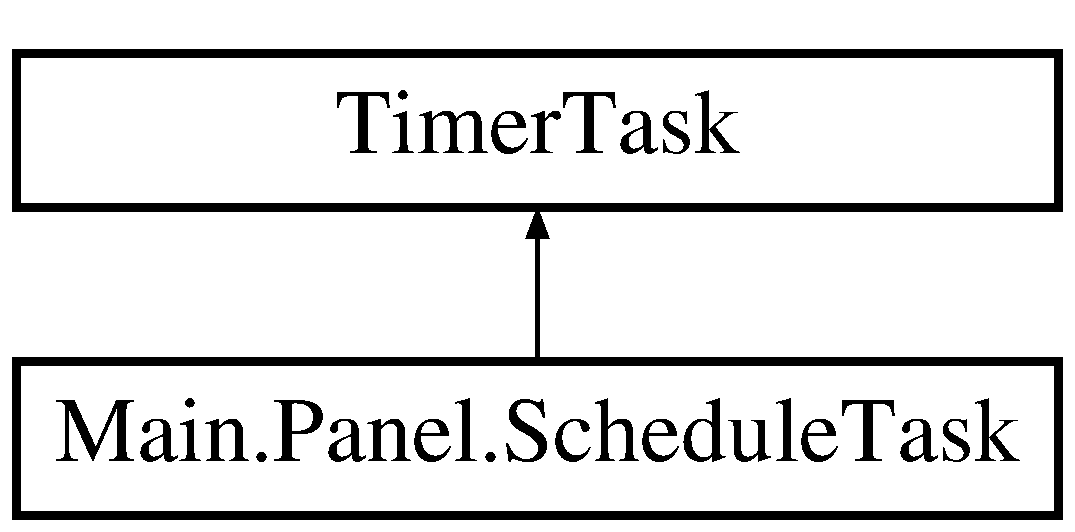
\includegraphics[height=2.000000cm]{class_main_1_1_panel_1_1_schedule_task}
\end{center}
\end{figure}
\subsection*{Public Member Functions}
\begin{DoxyCompactItemize}
\item 
void {\bfseries run} ()\hypertarget{class_main_1_1_panel_1_1_schedule_task_a5ff577b290e9615719387a147318872f}{}\label{class_main_1_1_panel_1_1_schedule_task_a5ff577b290e9615719387a147318872f}

\end{DoxyCompactItemize}


\subsection{Detailed Description}
Minden P\+E\+R\+I\+OD ms-\/ban meghívódik. A run() metódusával mozgatjuk az ütőt és ezáltal a labdát is. Mindeküzben figyeljük az esetleges ütözéseket, és újrarajzoljuk az ablak tartalmát. 

The documentation for this class was generated from the following file\+:\begin{DoxyCompactItemize}
\item 
E\+:/\+Egyetem/\+I\+I. ev/\+I. felev/\+Java/\+H\+F Break Bricks/src/\+Main/Panel.\+java\end{DoxyCompactItemize}

\hypertarget{class_main_1_1_panel_1_1_t_adapter}{}\section{Main.\+Panel.\+T\+Adapter Class Reference}
\label{class_main_1_1_panel_1_1_t_adapter}\index{Main.\+Panel.\+T\+Adapter@{Main.\+Panel.\+T\+Adapter}}
Inheritance diagram for Main.\+Panel.\+T\+Adapter\+:\begin{figure}[H]
\begin{center}
\leavevmode
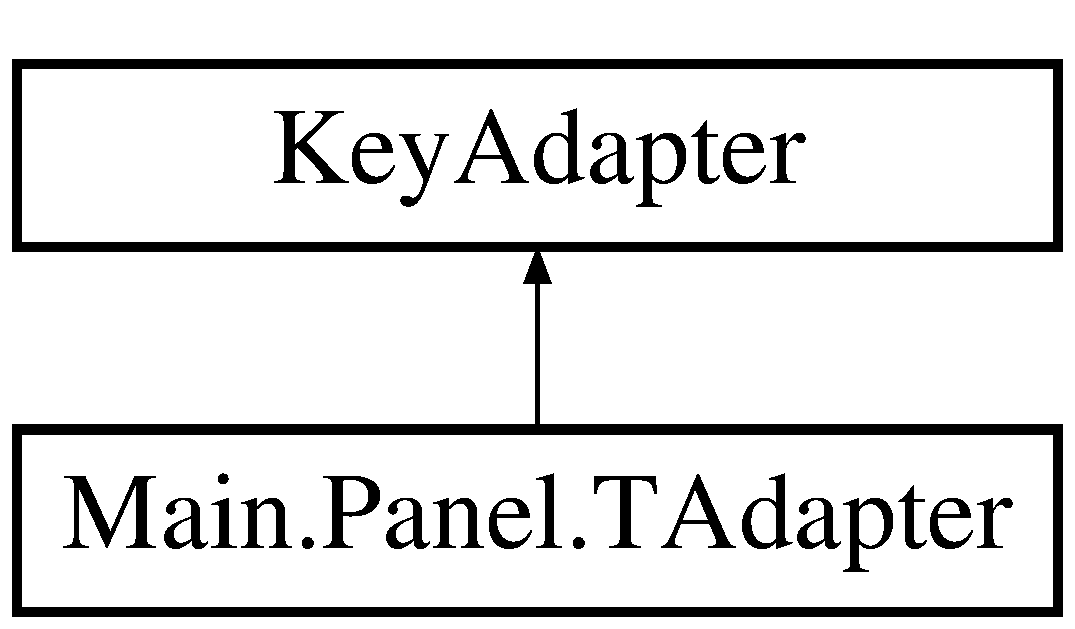
\includegraphics[height=2.000000cm]{class_main_1_1_panel_1_1_t_adapter}
\end{center}
\end{figure}
\subsection*{Public Member Functions}
\begin{DoxyCompactItemize}
\item 
void \hyperlink{class_main_1_1_panel_1_1_t_adapter_ac6ac1e979f5672e489ab65d4811ffcd1}{key\+Released} (Key\+Event event)
\item 
void \hyperlink{class_main_1_1_panel_1_1_t_adapter_a58164daef8b14a60ad738d22199acbfb}{key\+Pressed} (Key\+Event event)
\end{DoxyCompactItemize}


\subsection{Detailed Description}
Segédosztály, amely figyeli hogy mikor nyomjuk le és engedjük fel a paddle-\/t irányító gombot. 

\subsection{Member Function Documentation}
\index{Main\+::\+Panel\+::\+T\+Adapter@{Main\+::\+Panel\+::\+T\+Adapter}!key\+Pressed@{key\+Pressed}}
\index{key\+Pressed@{key\+Pressed}!Main\+::\+Panel\+::\+T\+Adapter@{Main\+::\+Panel\+::\+T\+Adapter}}
\subsubsection[{\texorpdfstring{key\+Pressed(\+Key\+Event event)}{keyPressed(KeyEvent event)}}]{\setlength{\rightskip}{0pt plus 5cm}void Main.\+Panel.\+T\+Adapter.\+key\+Pressed (
\begin{DoxyParamCaption}
\item[{Key\+Event}]{event}
\end{DoxyParamCaption}
)}\hypertarget{class_main_1_1_panel_1_1_t_adapter_a58164daef8b14a60ad738d22199acbfb}{}\label{class_main_1_1_panel_1_1_t_adapter_a58164daef8b14a60ad738d22199acbfb}
Meghívja a \hyperlink{class_main_1_1_paddle}{Paddle} osztály key\+Pressed osztályát. 
\begin{DoxyParams}{Parameters}
{\em event} & Key\+Event beépített osztály paramétere \\
\hline
\end{DoxyParams}
\index{Main\+::\+Panel\+::\+T\+Adapter@{Main\+::\+Panel\+::\+T\+Adapter}!key\+Released@{key\+Released}}
\index{key\+Released@{key\+Released}!Main\+::\+Panel\+::\+T\+Adapter@{Main\+::\+Panel\+::\+T\+Adapter}}
\subsubsection[{\texorpdfstring{key\+Released(\+Key\+Event event)}{keyReleased(KeyEvent event)}}]{\setlength{\rightskip}{0pt plus 5cm}void Main.\+Panel.\+T\+Adapter.\+key\+Released (
\begin{DoxyParamCaption}
\item[{Key\+Event}]{event}
\end{DoxyParamCaption}
)}\hypertarget{class_main_1_1_panel_1_1_t_adapter_ac6ac1e979f5672e489ab65d4811ffcd1}{}\label{class_main_1_1_panel_1_1_t_adapter_ac6ac1e979f5672e489ab65d4811ffcd1}
Meghívja a \hyperlink{class_main_1_1_paddle}{Paddle} osztály key\+Released osztályát. 
\begin{DoxyParams}{Parameters}
{\em event} & Key\+Event beépített osztály paramétere \\
\hline
\end{DoxyParams}


The documentation for this class was generated from the following file\+:\begin{DoxyCompactItemize}
\item 
E\+:/\+Egyetem/\+I\+I. ev/\+I. felev/\+Java/\+H\+F Break Bricks/src/\+Main/Panel.\+java\end{DoxyCompactItemize}

\hypertarget{classtest_1_1_test2}{}\section{test.\+Test2 Class Reference}
\label{classtest_1_1_test2}\index{test.\+Test2@{test.\+Test2}}
\subsection*{Public Member Functions}
\begin{DoxyCompactItemize}
\item 
void \hyperlink{classtest_1_1_test2_a7c5e762a59cf4dd38c6c7df81dcf9831}{Test\+Wizard\+Set\+And\+GetX} ()
\item 
void \hyperlink{classtest_1_1_test2_aa6bc4b81aed7d70c4670f3ec6fba0934}{Test\+Wizard\+Set\+And\+GetY} ()
\item 
void \hyperlink{classtest_1_1_test2_aea166c617674b555e0751052214498c0}{Test\+Ball\+Set\+And\+Get\+X\+Direction} ()
\item 
void \hyperlink{classtest_1_1_test2_a4f48c410ae21306ae516afdec411c878}{Test\+Ball\+Set\+And\+Get\+Y\+Direction} ()
\item 
void \hyperlink{classtest_1_1_test2_a12421d86d9961f7458de94356b09bfa4}{Record\+Read\+Test} ()  throws I\+O\+Exception 
\item 
void \hyperlink{classtest_1_1_test2_a85729314bfa16f727394157f74d252b9}{Test\+Brick\+Is\+Destroyed\+Andset\+Destroyed} ()
\end{DoxyCompactItemize}


\subsection{Detailed Description}
Created by Előd on 2016.\+11.\+29.. 

\subsection{Member Function Documentation}
\index{test\+::\+Test2@{test\+::\+Test2}!Record\+Read\+Test@{Record\+Read\+Test}}
\index{Record\+Read\+Test@{Record\+Read\+Test}!test\+::\+Test2@{test\+::\+Test2}}
\subsubsection[{\texorpdfstring{Record\+Read\+Test()}{RecordReadTest()}}]{\setlength{\rightskip}{0pt plus 5cm}void test.\+Test2.\+Record\+Read\+Test (
\begin{DoxyParamCaption}
{}
\end{DoxyParamCaption}
) throws I\+O\+Exception}\hypertarget{classtest_1_1_test2_a12421d86d9961f7458de94356b09bfa4}{}\label{classtest_1_1_test2_a12421d86d9961f7458de94356b09bfa4}
A Record osztály read\+Object() függcényének a tesztelése, amely egy fájlból olvas be adatokat, amennyiben a fájl létezik. Viszotn ha nem létezik a megadott nevű fájl, I\+O\+Exeptiont dob. 
\begin{DoxyExceptions}{Exceptions}
{\em I\+O\+Exception} & -\/ IO kivételt dob hiba esetén. \\
\hline
\end{DoxyExceptions}
\index{test\+::\+Test2@{test\+::\+Test2}!Test\+Ball\+Set\+And\+Get\+X\+Direction@{Test\+Ball\+Set\+And\+Get\+X\+Direction}}
\index{Test\+Ball\+Set\+And\+Get\+X\+Direction@{Test\+Ball\+Set\+And\+Get\+X\+Direction}!test\+::\+Test2@{test\+::\+Test2}}
\subsubsection[{\texorpdfstring{Test\+Ball\+Set\+And\+Get\+X\+Direction()}{TestBallSetAndGetXDirection()}}]{\setlength{\rightskip}{0pt plus 5cm}void test.\+Test2.\+Test\+Ball\+Set\+And\+Get\+X\+Direction (
\begin{DoxyParamCaption}
{}
\end{DoxyParamCaption}
)}\hypertarget{classtest_1_1_test2_aea166c617674b555e0751052214498c0}{}\label{classtest_1_1_test2_aea166c617674b555e0751052214498c0}
A Ball osztály set\+X\+Direction(), illetve get\+X\+Direction() függvényeinek tesztelése. \index{test\+::\+Test2@{test\+::\+Test2}!Test\+Ball\+Set\+And\+Get\+Y\+Direction@{Test\+Ball\+Set\+And\+Get\+Y\+Direction}}
\index{Test\+Ball\+Set\+And\+Get\+Y\+Direction@{Test\+Ball\+Set\+And\+Get\+Y\+Direction}!test\+::\+Test2@{test\+::\+Test2}}
\subsubsection[{\texorpdfstring{Test\+Ball\+Set\+And\+Get\+Y\+Direction()}{TestBallSetAndGetYDirection()}}]{\setlength{\rightskip}{0pt plus 5cm}void test.\+Test2.\+Test\+Ball\+Set\+And\+Get\+Y\+Direction (
\begin{DoxyParamCaption}
{}
\end{DoxyParamCaption}
)}\hypertarget{classtest_1_1_test2_a4f48c410ae21306ae516afdec411c878}{}\label{classtest_1_1_test2_a4f48c410ae21306ae516afdec411c878}
A Ball osztály set\+Y\+Direction(), illetve get\+Y\+Direction() függvényeinek tesztelése. \index{test\+::\+Test2@{test\+::\+Test2}!Test\+Brick\+Is\+Destroyed\+Andset\+Destroyed@{Test\+Brick\+Is\+Destroyed\+Andset\+Destroyed}}
\index{Test\+Brick\+Is\+Destroyed\+Andset\+Destroyed@{Test\+Brick\+Is\+Destroyed\+Andset\+Destroyed}!test\+::\+Test2@{test\+::\+Test2}}
\subsubsection[{\texorpdfstring{Test\+Brick\+Is\+Destroyed\+Andset\+Destroyed()}{TestBrickIsDestroyedAndsetDestroyed()}}]{\setlength{\rightskip}{0pt plus 5cm}void test.\+Test2.\+Test\+Brick\+Is\+Destroyed\+Andset\+Destroyed (
\begin{DoxyParamCaption}
{}
\end{DoxyParamCaption}
)}\hypertarget{classtest_1_1_test2_a85729314bfa16f727394157f74d252b9}{}\label{classtest_1_1_test2_a85729314bfa16f727394157f74d252b9}
A Brick osztály is\+Destroyed(), illetve set\+Destroyed() függvényeinek tesztelése. \index{test\+::\+Test2@{test\+::\+Test2}!Test\+Wizard\+Set\+And\+GetX@{Test\+Wizard\+Set\+And\+GetX}}
\index{Test\+Wizard\+Set\+And\+GetX@{Test\+Wizard\+Set\+And\+GetX}!test\+::\+Test2@{test\+::\+Test2}}
\subsubsection[{\texorpdfstring{Test\+Wizard\+Set\+And\+Get\+X()}{TestWizardSetAndGetX()}}]{\setlength{\rightskip}{0pt plus 5cm}void test.\+Test2.\+Test\+Wizard\+Set\+And\+GetX (
\begin{DoxyParamCaption}
{}
\end{DoxyParamCaption}
)}\hypertarget{classtest_1_1_test2_a7c5e762a59cf4dd38c6c7df81dcf9831}{}\label{classtest_1_1_test2_a7c5e762a59cf4dd38c6c7df81dcf9831}
A Wizard osztály set\+X(), illetve get\+X() függvényeinek tesztelése. \index{test\+::\+Test2@{test\+::\+Test2}!Test\+Wizard\+Set\+And\+GetY@{Test\+Wizard\+Set\+And\+GetY}}
\index{Test\+Wizard\+Set\+And\+GetY@{Test\+Wizard\+Set\+And\+GetY}!test\+::\+Test2@{test\+::\+Test2}}
\subsubsection[{\texorpdfstring{Test\+Wizard\+Set\+And\+Get\+Y()}{TestWizardSetAndGetY()}}]{\setlength{\rightskip}{0pt plus 5cm}void test.\+Test2.\+Test\+Wizard\+Set\+And\+GetY (
\begin{DoxyParamCaption}
{}
\end{DoxyParamCaption}
)}\hypertarget{classtest_1_1_test2_aa6bc4b81aed7d70c4670f3ec6fba0934}{}\label{classtest_1_1_test2_aa6bc4b81aed7d70c4670f3ec6fba0934}
A Wizard osztály set\+Y(), illetve get\+Y() függvényeinek tesztelése. 

The documentation for this class was generated from the following file\+:\begin{DoxyCompactItemize}
\item 
E\+:/\+Egyetem/\+I\+I. ev/\+I. felev/\+Java/\+H\+F Break Bricks/test/test/Test2.\+java\end{DoxyCompactItemize}

\hypertarget{class_main_1_1_wizard}{}\section{Main.\+Wizard Class Reference}
\label{class_main_1_1_wizard}\index{Main.\+Wizard@{Main.\+Wizard}}
Inheritance diagram for Main.\+Wizard\+:\begin{figure}[H]
\begin{center}
\leavevmode
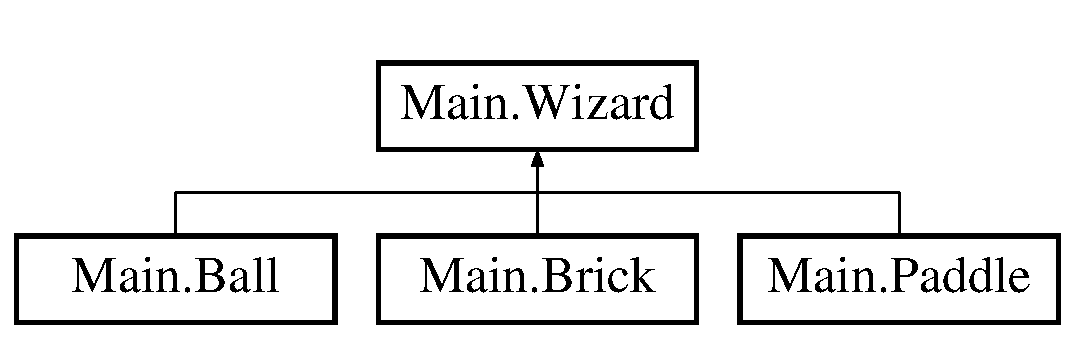
\includegraphics[height=2.000000cm]{class_main_1_1_wizard}
\end{center}
\end{figure}
\subsection*{Public Member Functions}
\begin{DoxyCompactItemize}
\item 
void \hyperlink{class_main_1_1_wizard_aa4b5c7faf39649ed8fb1fb33cc3788e6}{setX} (int x)
\item 
void \hyperlink{class_main_1_1_wizard_a4c5d8c80ab66a0d2fa140ac5052f2d02}{setY} (int y)
\item 
int \hyperlink{class_main_1_1_wizard_af96f444dd5a2c9c62dfd8fdcbfd879f0}{getX} ()
\item 
int \hyperlink{class_main_1_1_wizard_a718fbfb8924f38028d230fd094c3aaf4}{getY} ()
\item 
int \hyperlink{class_main_1_1_wizard_a0c586454e8d579cb317f180a98755add}{get\+Width} ()
\item 
int \hyperlink{class_main_1_1_wizard_a88842db1cff1b208b0451456fbfa3593}{get\+Height} ()
\end{DoxyCompactItemize}
\subsection*{Public Attributes}
\begin{DoxyCompactItemize}
\item 
Image {\bfseries image}\hypertarget{class_main_1_1_wizard_a7abcdd7a22fc8f92f69cfa19700aa6cd}{}\label{class_main_1_1_wizard_a7abcdd7a22fc8f92f69cfa19700aa6cd}

\end{DoxyCompactItemize}
\subsection*{Protected Attributes}
\begin{DoxyCompactItemize}
\item 
int {\bfseries x}\hypertarget{class_main_1_1_wizard_a6f623e01fc07da97597ba27c34a4974e}{}\label{class_main_1_1_wizard_a6f623e01fc07da97597ba27c34a4974e}

\item 
int {\bfseries y}\hypertarget{class_main_1_1_wizard_acec507c2727a6a2a5976c499444cd48f}{}\label{class_main_1_1_wizard_acec507c2727a6a2a5976c499444cd48f}

\item 
int {\bfseries iwidth}\hypertarget{class_main_1_1_wizard_ae710f20e4aba920201fd0cf66c8f71ab}{}\label{class_main_1_1_wizard_ae710f20e4aba920201fd0cf66c8f71ab}

\item 
int {\bfseries iheight}\hypertarget{class_main_1_1_wizard_acf427428af494d712b4f9f6d5adce18d}{}\label{class_main_1_1_wizard_acf427428af494d712b4f9f6d5adce18d}

\end{DoxyCompactItemize}


\subsection{Detailed Description}
A \hyperlink{class_main_1_1_wizard}{Wizard}(magyarul\+: varázsló, későbbiekben is fogok rá így hivatkozni) osztály egy segédosztály, amit felhasználnak az elemek osztályai. Itt vannak azok az változók és metódusok, amiket a \hyperlink{class_main_1_1_brick}{Brick}, \hyperlink{class_main_1_1_ball}{Ball}, \hyperlink{class_main_1_1_paddle}{Paddle} osztályok, valamint objektumok egyaránt felhasználnak. Úgymond egy segédosztály ami megkönnyti a többi osztály működését, és nem kell ezeketa metódusokat minden osztályba külön definiálni, megkönnyítve a program átláthatóságát és fejleszthetőségét. 

\subsection{Member Function Documentation}
\index{Main\+::\+Wizard@{Main\+::\+Wizard}!get\+Height@{get\+Height}}
\index{get\+Height@{get\+Height}!Main\+::\+Wizard@{Main\+::\+Wizard}}
\subsubsection[{\texorpdfstring{get\+Height()}{getHeight()}}]{\setlength{\rightskip}{0pt plus 5cm}int Main.\+Wizard.\+get\+Height (
\begin{DoxyParamCaption}
{}
\end{DoxyParamCaption}
)}\hypertarget{class_main_1_1_wizard_a88842db1cff1b208b0451456fbfa3593}{}\label{class_main_1_1_wizard_a88842db1cff1b208b0451456fbfa3593}
A hozzá tartozó kép magasságát határozza meg. \begin{DoxyReturn}{Returns}
iheight Visszatér az iheight értékkel 
\end{DoxyReturn}
\index{Main\+::\+Wizard@{Main\+::\+Wizard}!get\+Width@{get\+Width}}
\index{get\+Width@{get\+Width}!Main\+::\+Wizard@{Main\+::\+Wizard}}
\subsubsection[{\texorpdfstring{get\+Width()}{getWidth()}}]{\setlength{\rightskip}{0pt plus 5cm}int Main.\+Wizard.\+get\+Width (
\begin{DoxyParamCaption}
{}
\end{DoxyParamCaption}
)}\hypertarget{class_main_1_1_wizard_a0c586454e8d579cb317f180a98755add}{}\label{class_main_1_1_wizard_a0c586454e8d579cb317f180a98755add}
Visszatér az iwidth értékkel, ami a hozzá tartozó kép szélességét határozza meg. \begin{DoxyReturn}{Returns}
iwidth 
\end{DoxyReturn}
\index{Main\+::\+Wizard@{Main\+::\+Wizard}!getX@{getX}}
\index{getX@{getX}!Main\+::\+Wizard@{Main\+::\+Wizard}}
\subsubsection[{\texorpdfstring{get\+X()}{getX()}}]{\setlength{\rightskip}{0pt plus 5cm}int Main.\+Wizard.\+getX (
\begin{DoxyParamCaption}
{}
\end{DoxyParamCaption}
)}\hypertarget{class_main_1_1_wizard_af96f444dd5a2c9c62dfd8fdcbfd879f0}{}\label{class_main_1_1_wizard_af96f444dd5a2c9c62dfd8fdcbfd879f0}
Visszatér az aktuális x paraméterrel. \begin{DoxyReturn}{Returns}
x koordináta értéke 
\end{DoxyReturn}
\index{Main\+::\+Wizard@{Main\+::\+Wizard}!getY@{getY}}
\index{getY@{getY}!Main\+::\+Wizard@{Main\+::\+Wizard}}
\subsubsection[{\texorpdfstring{get\+Y()}{getY()}}]{\setlength{\rightskip}{0pt plus 5cm}int Main.\+Wizard.\+getY (
\begin{DoxyParamCaption}
{}
\end{DoxyParamCaption}
)}\hypertarget{class_main_1_1_wizard_a718fbfb8924f38028d230fd094c3aaf4}{}\label{class_main_1_1_wizard_a718fbfb8924f38028d230fd094c3aaf4}
Visszatér az aktuális y paraméterrel. \begin{DoxyReturn}{Returns}
y koordináta értéke 
\end{DoxyReturn}
\index{Main\+::\+Wizard@{Main\+::\+Wizard}!setX@{setX}}
\index{setX@{setX}!Main\+::\+Wizard@{Main\+::\+Wizard}}
\subsubsection[{\texorpdfstring{set\+X(int x)}{setX(int x)}}]{\setlength{\rightskip}{0pt plus 5cm}void Main.\+Wizard.\+setX (
\begin{DoxyParamCaption}
\item[{int}]{x}
\end{DoxyParamCaption}
)}\hypertarget{class_main_1_1_wizard_aa4b5c7faf39649ed8fb1fb33cc3788e6}{}\label{class_main_1_1_wizard_aa4b5c7faf39649ed8fb1fb33cc3788e6}
Beállítja az x paramétert a megadott értékre. 
\begin{DoxyParams}{Parameters}
{\em x} & az x koordináta értéke \\
\hline
\end{DoxyParams}
\index{Main\+::\+Wizard@{Main\+::\+Wizard}!setY@{setY}}
\index{setY@{setY}!Main\+::\+Wizard@{Main\+::\+Wizard}}
\subsubsection[{\texorpdfstring{set\+Y(int y)}{setY(int y)}}]{\setlength{\rightskip}{0pt plus 5cm}void Main.\+Wizard.\+setY (
\begin{DoxyParamCaption}
\item[{int}]{y}
\end{DoxyParamCaption}
)}\hypertarget{class_main_1_1_wizard_a4c5d8c80ab66a0d2fa140ac5052f2d02}{}\label{class_main_1_1_wizard_a4c5d8c80ab66a0d2fa140ac5052f2d02}
Beállítja az y paramétert a megadott értékre. 
\begin{DoxyParams}{Parameters}
{\em y} & az y koordináta értéke \\
\hline
\end{DoxyParams}


The documentation for this class was generated from the following file\+:\begin{DoxyCompactItemize}
\item 
E\+:/\+Egyetem/\+I\+I. ev/\+I. felev/\+Java/\+H\+F Break Bricks/src/\+Main/Wizard.\+java\end{DoxyCompactItemize}

%--- End generated contents ---

% Index
\backmatter
\newpage
\phantomsection
\clearemptydoublepage
\addcontentsline{toc}{chapter}{Index}
\printindex

\end{document}
